% !TEX root = ../main.tex

%************************************************
\chapter{Quasar-driven galaxy-wide outflows in ionised gas}
\chaptermark{Galaxy-wide outflows}

\label{ch:nlr} 
%************************************************

\section{[\ion{O}{III}] as a probe of quasar-driven outflows}

X-ray and ultra-violet spectroscopy has revealed high-velocity outflows to be nearly ubiquitous in high accretion rate quasars.
Strong evidence for high-velocity outflows in the vicinity of quasars include BALs, NALs and blueshifted emission-lines. 
These observations suggest that the energy released by quasars can have a dramatic effect on their immediate environments. 

Quasars driving powerful outflows over galactic scales is a central tenet of galaxy evolution models involving `quasar feedback' \citep[e.g.][]{silk98,springel05,bower06}.
In recent years, a huge amount of resources have been devoted to searching for observational evidence of this phenomenon.  
This has resulted in recent detections of outflows in quasar-host galaxies using tracers of atomic, molecular, and ionised gas \citep[e.g.][]{nesvadba06,arav08,nesvadba08,moe09,alexander10,dunn10,feruglio10,nesvadba10,alatalo11,cano-diaz12,harrison12,harrison14,cimatti13,rupke13,veilleux13,cicone14,nardini15}.  

One particularly successful technique has been to use forbidden quasar emission-lines to probe the dynamical state of the ionised gas extended over kilo-parsec scales in quasar host-galaxies. 
Because of its high equivalent width, [\ion{O}{III}]\l$5008$ is the most studied of the narrow quasar emission-lines. 
The [\ion{O}{III}] emission is found to consist of two distinct components: a narrow, `core' component, with a velocity close to the systemic redshift of the host-galaxy, and a broader `wing' component, which is normally blueshifted. 
The core component is dominated by the gravitational potential of the host-galaxy.
However, the velocity-width of the wing is much too broad for the gas to be in dynamical equilibrium with the host-galaxy \citep[e.g.][]{liu13} and the general consensus is that it is tracing high-velocity outflowing gas. The receding side of the outflow may be obscured due to the presence of dust, either in the outflow or elsewhere, and so only the near-side of the outflow, which is blueshifted, is observed. 
The relative balance between the core and wing components varies significantly from object to object, and governs the width and asymmetry of the overall [\ion{O}{III}] emission profile \citep[e.g.][]{shen14}. 

Observations of broad velocity-widths and blueshifts in narrow emission-lines stretch back several decades \citep[e.g.][]{weedman70,stockton76,heckman81,veron81,feldman82,heckman84,vrtilek85,whittle85,boroson92}. 
However, these studies rely on small samples, which are often unrepresentative of the properties of the quasar population. 
More recently, the advent of large optical spectroscopic surveys (e.g. SDSS) have facilitated studies of the NLR in tens of thousands of quasars \citep[e.g.][]{boroson05,greene05a,zhang11,mullaney13,zakamska14,shen14}. 
This has provided constraints on the prevalence and drivers of ionised outflows.   
At the same time, there is strong evidence from spatially resolved spectroscopy that these outflows are extended over galaxy scales \citep[e.g.][]{greene09,greene11,harrison12,hainline13,harrison14}. 

However, these studies do not cover the redshift range when star formation and BH accretion peaked ($2 \lesssim z \lesssim 4$), which is when the $M_{\text{BH}}-\sigma$ relation is thought to have been established. 
At these redshifts bright optical emission-lines including the [\ion{O}{III}] doublet are redshifted to near-infrared wavelengths, where observations are far more challenging. 
As a consequence, studies at high redshifts have typically relied on relatively small numbers of objects.
These studies find [\ion{O}{III}] to be broader in more luminous quasars, with velocity-widths $\gtrsim1000$\,\kms\, common \citep[e.g.][]{netzer04,kim13,brusa15,shen16a}.  
These findings suggest that quasar efficiency in driving galaxy-wide outflows increases with luminosity \citep[e.g.][]{netzer04,nesvadba08,kim13,brusa15,carniani15,perna15,bischetti16}. 
The fraction of objects with very weak [\ion{O}{III}] emission also appears to increase with redshift and/or luminosity \citep[e.g.][]{netzer04}. 

In this chapter, we analyse the [\ion{O}{III}] properties of a sample of $354$ high-luminosity, redshift $1.5 < z < 4$ quasars.
To date, this is the largest study of the NLR properties of high redshift quasars. 

\section[Sample construction]{Constructing a sample with [\ion{O}{III}] spectra}

From our near-infrared spectroscopic catalogue (Chapter~\ref{ch:nirsample}), we have selected $354$ quasars which have spectra covering the [\ion{O}{III}] doublet. 
The broad Balmer \hb line has also been observed for all but two of the sample. 
For $165$ quasars, the spectra extend to the broad \ha emission-line at $6565$\,\AA, and in $260$ objects optical spectra, including \ion{C}{IV}, are also available (mostly from SDSS/BOSS). 
The sample covers a wide range in redshifts ($1.5 \lesssim z \lesssim 4$) and luminosities ($45.5 \lesssim \log L_{\text{Bol}} \lesssim 49$\,\ergs). 
The spectrographs and telescopes used to obtain the near-infrared spectra are summarised in Table~\ref{tab:specnums_ch4}.

\begin{table}
  \centering
  \footnotesize 
    \begin{tabular}{ccc} 
    \hline
    Spectrograph & Telescope & Number \\
                 &           & \\
    \hline
    FIRE         & MAGELLAN  & $31$ \\
    GNIRS        & GEMINI-N  & $28$ \\
    ISAAC        & VLT       & $7$ \\
    LIRIS        & WHT       & $7$ \\
    NIRI         & GEMINI-N  & $29$ \\
    NIRSPEC      & Keck II   & $3$ \\
    SINFONI      & VLT       & $80$ \\
    SOFI         & NTT       & $76$ \\
    TRIPLESPEC   & ARC-$3.5$m  & $27$ \\
    TRIPLESPEC   & P$200$      & $45$ \\
    XSHOOTER     & VLT       & $21$ \\
    \hline
    \multicolumn{2}{c}{Total} & $354$ \\
    \hline
    \end{tabular}
    \caption[{The numbers of quasars with [\ion{O}{III}] line measurements and the spectrographs and telescopes used to obtain the near-infrared spectra.}]{The numbers of quasars with [\ion{O}{III}] line measurements and the spectrographs and telescopes used to obtain the near-infrared spectra.}
  \label{tab:specnums_ch4}
\end{table} 

\section{Spectral measurements}

In this section, the procedure we use to measure emission-line properties is described.  
Our approach is to model the \hbns/[\ion{O}{III}] complex using a power-law continuum, an empirical \ion{Fe}{II} template (taken from \citealt{boroson92}) and multiple Gaussian components.
Non-parametric properties are then derived from the best-fitting model. 
This approach, which is commonly adopted in the literature \citep[e.g.][]{shen11,shen12,shen16a}, is more robust when analysing spectra with limited S/N (in comparison to measuring line properties directly from the data) and allows adjacent emission-lines to be de-blended.

The modelling of \ha (used in this chapter to estimate the quasar systemic redshift) is also described.   
\ion{C}{IV} emission-line properties (used to infer the strength of BLR outflows) are taken directly from Chapter~\ref{ch:bhmass}. 

\subsection{Transforming spectra to rest-frame wavelengths}

Before a spectrum can be modelled, it must first be transformed to the rest-frame of the quasar.  
The redshift used in this transformation is either derived from the peak of the broad \ha emission ($\sim40$ per cent of our sample), from the peak of the broad \hb emission ($\sim40$ per cent) or from the peak of the narrow [\ion{O}{III}] emission ($20$ per cent).
The rest-frame transformation is only required to be accurate to within $\sim1000$\,\kms\, of the true systemic redshift for our fitting procedure to function. 
In later sections, more precise estimates of the systemic redshift will be calculated using our parametric model fits. 

\subsection{Removing \ion{Fe}{II} emission}
\label{sec:ch4-fe-removal}

\begin{figure}
    \centering
    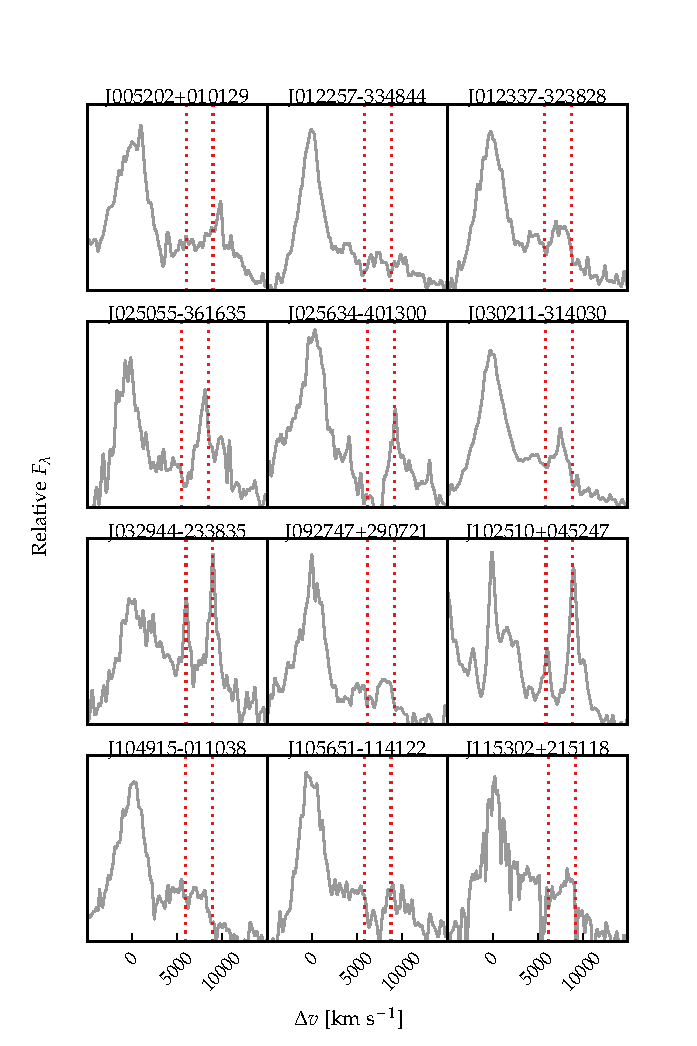
\includegraphics[width=\columnwidth]{figures/chapter04/example_spectrum_grid_extreme_fe_1.pdf} 
    \caption[{Spectra of the $24$ objects for which significant \ion{Fe}{II} emission is still present following our \ion{Fe}{II}-subtraction procedure.}]{Spectra of the $24$ objects for which significant \ion{Fe}{II} emission is still present following our \ion{Fe}{II}-subtraction procedure. Spectra have been smoothed via convolution with a $100$\,\kms\, Gaussian kernel. The vertical lines indicate the expected positions of the [\ion{O}{III}] doublet (which is generally very weak in these objects) with the systemic redshift defined using the peak of the broad \hb emission.}     
    \label{fig:bad_fe}
\end{figure}

\begin{figure}
\ContinuedFloat
    \centering
    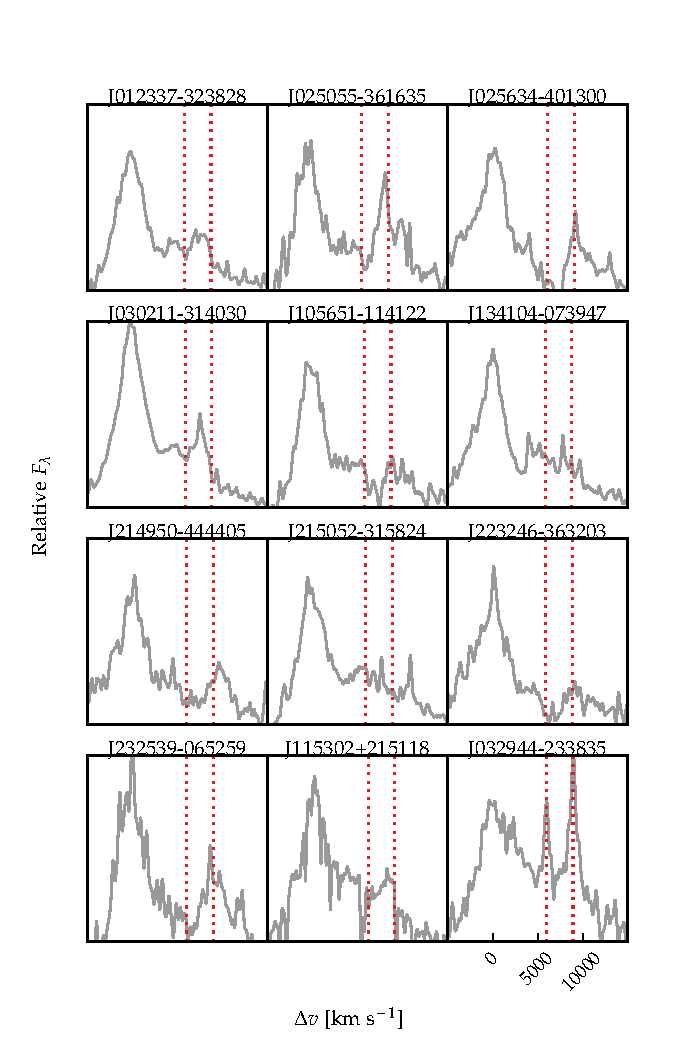
\includegraphics[width=\columnwidth]{figures/chapter04/example_spectrum_grid_extreme_fe_2.pdf} 
    \caption[]{Continued.}     
\end{figure}

Before \hbns/[\ion{O}{III}] is modelled, we first model and subtract the nearby continuum and \ion{Fe}{II} emission using the procedure described in Chapter~\ref{ch:bhmass}. 
We encountered $24$ objects for which the procedure failed to adequately remove the \ion{Fe}{II} emission from the spectra (Figure~\ref{fig:bad_fe}).  
In these objects the relative strengths of the \ion{Fe}{II} lines differ significantly from those of I Zw $1$, on which the \citet{boroson92} \ion{Fe}{II} template we use is based. 
The residual \ion{Fe}{II} emission is at rest-frame wavelengths very close to the laboratory wavelengths of the [\ion{O}{III}] doublet, which is generally very weak in these objects. 
As a result, the [\ion{O}{III}] line parameters we derive for these objects are unreliable. 
These objects are therefore flagged and excluded from our analysis in the remainder of this chapter (leaving $330$ objects in our sample). 

To illustrate the importance of the \ion{Fe}{II} subtraction procedure in reliably measuring [\ion{O}{III}] emission properties, we consider the object J$223819$-$092106$ (shown bottom row, centre in Figure~\ref{fig:bad_fe}). 
This object was also analysed by \citet{shen16a}, who reported the [\ion{O}{III}] emission to have an extreme redshift ($\sim7500$\,\kms) relative to the \citet{hewett10} systemic redshift.
However, our analysis suggests that the emission which was modelled by \citet{shen16a} as [\ion{O}{III}] is more likely to be poorly-subtracted \ion{Fe}{II}.  

\subsection{Modelling \hbns/[\ion{O}{III}]}
\label{sec:oiiimodel}

\begin{table}
  \centering
  \footnotesize 
    \begin{tabular}{ccc} 
    \hline
    Model & Fix centroids? & Number \\
    \hline
    $2$ broad Gaussians + $1$ narrow Gaussian & No & $9$ \\
    $2$ broad Gaussians & No  &  $295$ \\
    $2$ broad Gaussians & Yes &  $39$ \\
    $1$ broad Gaussian  & N/A &  $9$ \\
    \hline
    \end{tabular}
    \caption[{Summary of models used to fit the \hb emission, and the number of quasars to which each model is applied.}]{Summary of models used to fit the \hb emission, and the number of quasars to which each model is applied.}
  \label{tab:hbmod}
\end{table} 

In general, \hb is modelled with two Gaussians with non-negative amplitudes and FWHM greater than $1200$\,\kms.
In nine objects \hb is modelled with a single Gaussian and in $39$ objects \hb is modelled with two Gaussians, but the velocity centroids of the two Gaussians are constrained to be equal. 
These spectra generally have low S/N, and adding extra freedom to the model does not significantly decrease the  reduced-$\chi^2$.
In addition there are cases where the blue wing of the \hb emission is below the lower wavelength limit of the spectra; in these cases models with more freedom are insufficiently constrained by the data.    

Contributions to the \hb emission from the NLR is generally weak in our sample, and an additional Gaussian component to model this emission is not required for the vast majority of objects. 
In nine objects features in the model - data residuals suggest that a narrow emission component is significant, and an additional narrow Gaussian is included in the model for these quasars. 
If the NLR contribution to the \hb emission is significant in more of our sample, then measures of the \hb velocity-width will be biased to lower values. 
However, our systemic redshift estimates that use the peak of the \hb emission (Section~\ref{sec:ch4_redshifts}) will not be affected. 
The \hb models, and the numbers of quasars to which each model is applied, are summarised in Table~\ref{tab:hbmod}. 

Each component of the [\ion{O}{III}] doublet is fit with one or two Gaussians, depending on the fractional reduced-$\chi^2$ difference between the one- and two-component models. 
Concretely, if the addition of the second Gaussian decreases the reduced-$\chi^2$ by more than $5$ per cent then the double-Gaussian model is accepted.
One hundred and twenty-eight spectra are fit with a single Gaussian and $140$ with two Gaussians. 
The peak flux ratio of the [\ion{O}{III}] $4960$\,\AA\, and $5008$\,\AA\, components are fixed at the expected $1$:$3$ ratio and the width and velocity offsets are set to be equal\footnote{For J$003136$+$003421$, a significantly better fit ($\Delta \chi^2_{\nu} \sim 25\%$) is obtained when the peak flux ratio constraint is relaxed; the peak ratio of the best-fitting model is $1$:$2.13$.}.

In $62$ objects with very weak [\ion{O}{III}] (mean $\text{EQW}\sim2$\,\AA) we find that the Gaussian model has a tendency to fit features to the noise. 
This can lead to large errors on the [\ion{O}{III}] line properties. 
To avoid this problem, we instead fit a fixed [\ion{O}{III}] template (FWHM $\simeq900$\,\kms) to the spectra, with the normalisation of this template the only free-parameter in the fit.
This template is generated by running our line-fitting routine on a median composite spectrum that we have constructed from the $268$ quasars with reliable [\ion{O}{III}] line measurements.  
The spectra used to construct the composite were first de-redshifted and continuum- and \ion{Fe}{II}-subtracted.

The models we use to fit [\ion{O}{III}], and the numbers of quasars to which each model is applied, are summarised in Table~\ref{tab:oiiimod}.

\begin{table}
  \centering
  \footnotesize 
    \begin{tabular}{cc} 
    \hline
    Model & Number \\
    \hline
    $2$ Gaussians &  $140$ \\
    $1$ Gaussian  &  $128$ \\
    Template &  $62$ \\
    \hline
    \end{tabular}
    \caption[{Summary of models used to fit the [\ion{O}{III}] emission, and the number of quasars to which each model is applied.}]{Summary of models used to fit the [\ion{O}{III}] emission, and the number of quasars to which each model is applied.}
  \label{tab:oiiimod}
\end{table} 

In Figure~\ref{fig:example_spectrum_grid} we show example fits to eight objects. 
The median reduced-$\chi^2$ value in the whole sample is $1.31$ and, in general, there are no strong features observable in the spectrum-minus-model residuals.

\begin{figure}
    \centering
    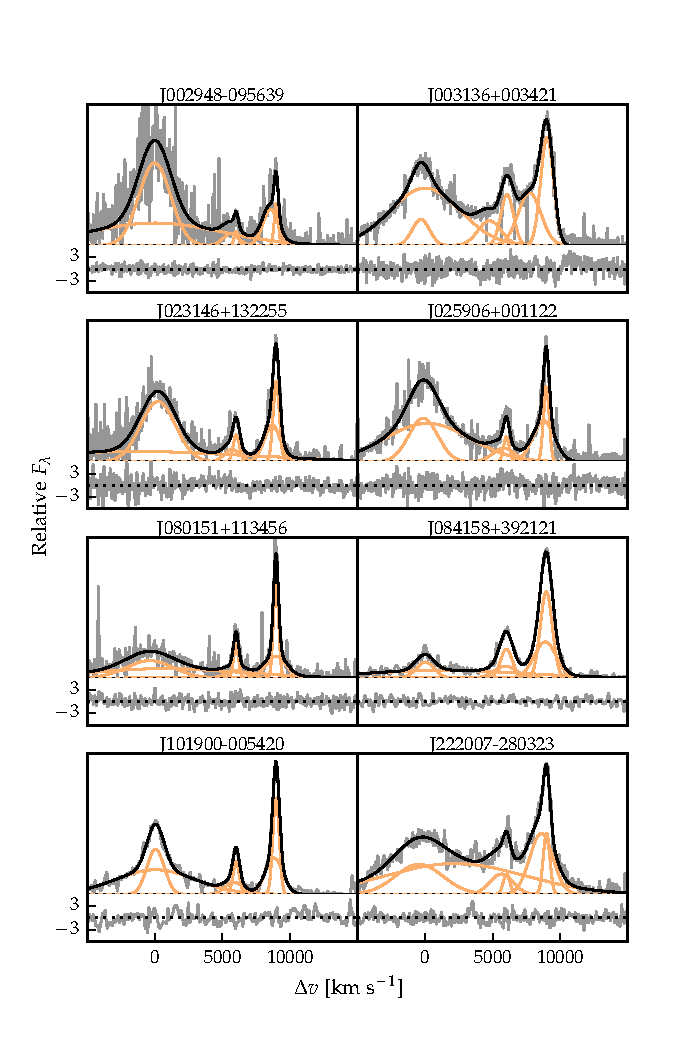
\includegraphics[width=\textwidth]{figures/chapter04/example_spectrum_grid.pdf} 
    \caption[{Example model fits to the \hbns/[\ion{O}{III}] emission in eight quasars.}]{Example model fits to the continuum- and \ion{Fe}{II}-subtracted \hbns/[\ion{O}{III}] emission in eight quasars. The data is shown in grey, the best-fitting model in black, and the individual model components in orange. The peak of the [\ion{O}{III}] emission is used to set the redshift, and $\Delta{v}$ is the velocity shift from the rest-frame transition wavelength of \hbns. Below each spectrum we plot the data-minus-model residuals, scaled by the errors on the fluxes.}     
    \label{fig:example_spectrum_grid}
\end{figure}

\subsection{Modelling \hans}
\label{sec:hamodel}

\begin{table}
  \centering
  \footnotesize 
    \begin{tabular}{cccc} 
    \hline
    Model     & Components & Fix centroids? & Number \\
    \hline
    1        & $1$ broad Gaussian  & N/A &  $8$ \\
    2        & $2$ broad Gaussians & Yes &  $47$ \\
    3        & $2$ broad Gaussians & No  &  $20$ \\
    4        & $2$ broad Gaussians + narrow Gaussians & Yes & $42$ \\
    5        & $2$ broad Gaussians + narrow Gaussians & No  & $48$ \\
    \hline
    \end{tabular}
    \caption[{Summary of models used to fit the \ha emission, and the number of quasars to which each model is applied.}]{Summary of models used to fit the \ha emission, and the number of quasars to which each model is applied.}
  \label{tab:hamod}
\end{table} 

There are $165$ quasars in our sample with spectra covering the \ha emission-line. 
In Section~\ref{sec:ch4_redshifts}, we use the peak of the \ha emission as one estimate of the quasar systemic redshift. 
In this section, we describe how the \ha emission was modelled. 

The continuum emission is first modeled and subtracted using the procedure described in Section~\ref{sec:ha}. 
We then test five different models with increasing degrees of freedom to model the \ha emission. 
The models are summarised in Table~\ref{tab:hamod}. 
They are (1) a single broad Gaussian; (2) two broad Gaussians with identical velocity centroids; (3) two broad Gaussians with different velocity centroids; (4) two broad Gaussians with identical velocity centroids, and additional narrower Gaussians to model narrow \ha emission, and the narrow components of [\ion{N}{II}]\ll$6548,6584$ and [\ion{S}{II}]\ll$6717,6731$; (5) two broad Gaussians with different velocity centroids, and additional narrower Gaussians. 
If used, the width and velocity of all narrow components are set to be equal in the fit, and the relative flux ratio of the two [\ion{N}{II}] components is fixed at the expected value of $2.96$.

In order to determine which model is selected for each spectrum we use the following procedure.  
Each of the five models are fit to every spectrum and the reduced-$\chi^2$ recorded.
Initially, the model with the smallest reduced-$\chi^2$ is selected. 
We then measure how the reduced-$\chi^2$ changes as the complexity of the model is decreased (i.e. considering the models in Table~\ref{tab:hamod} in descending order). 
If using the simpler model results in an increase in the reduced-$\chi^2$ which is less than $10$ per cent relative to the best fitting model, then the simpler model is selected.  

\subsection{Deriving emission-line properties from the best-fitting models}

\begin{figure}[t!]
    \centering
    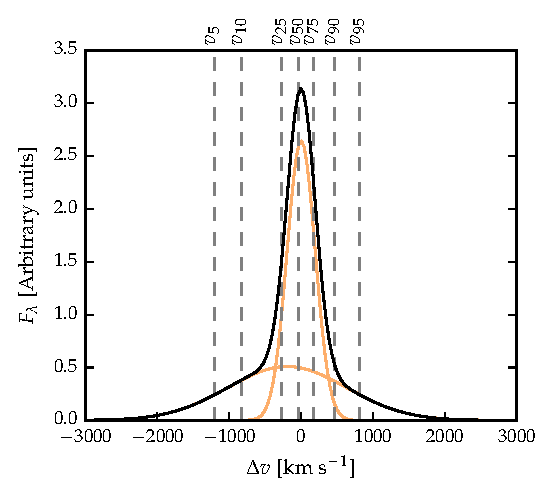
\includegraphics[width=0.8\textwidth]{figures/chapter04/example_oiii.pdf} 
    \caption[{Non-parametric measures of the [\ion{O}{III}] velocity-profile.}]{Non-parametric measures of the [\ion{O}{III}] velocity-profile, as described in the text.}     
    \label{fig:example_oiii}
\end{figure}

All [\ion{O}{III}] line properties are derived from the [\ion{O}{III}]\l$5008$ peak, but, as described above, the kinematics of [\ion{O}{III}]\l$4960$ are constrained to be identical in our fitting routine. 

We do not attach any physical meaning to the individual Gaussian components used in the model. 
Decomposing the [\ion{O}{III}] emission into a narrow component at the systemic redshift and a lower-amplitude, blueshifted broad component is often highly degenerate and dependent on the spectral S/N and resolution. 
Furthermore, there is no theoretical justification that the broad component should have a Gaussian profile.  

We therefore choose to characterize the [\ion{O}{III}] line profile using a number of non-parametric measures, which are commonly used in the literature \citep[e.g.][]{whittle85,zakamska14,zakamska16}. 
A normalised cumulative velocity distribution is constructed from the best-fitting model, from which the velocities below which $5$, $10$, $25$, $50$, $75$, $90$, and $95$ per cent of the total flux accumulates can be calculated. 
These velocities are then adjusted so that the peak of the [\ion{O}{III}] emission is at $0$\,\kms. 
The [\ion{O}{III}] velocities for an example model are shown in Figure~\ref{fig:example_oiii} 

We calculate the velocity-width containing $90$ per cent of the flux $w_{90}$ by rejecting $5$ per cent of the flux in the blue and red wings of the profile ($w_{90}\equiv v_{95} - v_{5}$).
We also calculate $w_{80}$ ($\equiv v_{90} - v_{10}$) and $w_{50}$ ($\equiv v_{75} - v_{25}$).
$w_{90}$ is relatively most sensitive to the flux in the wings of the line, whereas $w_{50}$ is relatively most sensitive to the flux in the core.  
In terms of the FWHM, $w_{50} \simeq \text{FWHM} / 1.746$, $w_{80} \simeq \text{FWHM} / 0.919$, $w_{90} \simeq \text{FWHM} / 0.716$, assuming a Gaussian line profile.  


\begin{table}
  \centering
  \footnotesize
  \centering
    \begin{tabular}{cccc} 
    \hline
    Column & Name & Units & Description \\ 
    \hline
    1 & UID & & Catalogue name \\
    2 & OIII\_V$5$ & \kms & [\ion{O}{III}] $v_{5}$ \\
    3 & OIII\_V$5$\_ERR & \kms & \\
    4 & OIII\_V$10$ & \kms & [\ion{O}{III}] $v_{10}$ \\
    5 & OIII\_V$10$\_ERR & \kms &  \\
    6 & OIII\_V$25$ & \kms & [\ion{O}{III}] $v_{25}$ \\
    7 & OIII\_V$25$\_ERR & \kms &  \\
    8 & OIII\_V$50$ & \kms & [\ion{O}{III}] $v_{50}$ \\
    9 & OIII\_V$50$\_ERR & \kms &  \\
    10 & OIII\_V$75$ & \kms & [\ion{O}{III}] $v_{75}$ \\
    11 & OIII\_V$75$\_ERR & \kms &  \\
    12 & OIII\_V$90$ & \kms & [\ion{O}{III}] $v_{90}$ \\
    13 & OIII\_V$90$\_ERR & \kms &  \\
    14 & OIII\_V$95$ & \kms & [\ion{O}{III}] $v_{95}$ \\
    15 & OIII\_V$95$\_ERR & \kms &  \\
    16 & OIII\_Z & & [\ion{O}{III}] redshift \\
    17 & OIII\_Z\_ERR & &  \\
    18 & OIII\_W$50$ & \kms & [\ion{O}{III}] $w_{50}$ \\
    19 & OIII\_W$50$\_ERR & \kms &  \\
    20 & OIII\_W$80$ & \kms & [\ion{O}{III}] $w_{80}$ \\
    21 & OIII\_W$80$\_ERR & \kms & \\
    22 & OIII\_W$90$ & \kms & [\ion{O}{III}] $w_{90}$ \\
    23 & OIII\_W$90$\_ERR & \kms & \\
    24 & OIII\_A & & [\ion{O}{III}] asymmetry \\
    25 & OIII\_A\_ERR & & \\
    26 & OIII\_EQW & \AA & [\ion{O}{III}] EQW \\
    27 & OIII\_EQW\_ERR & \AA & \\
    28 & OIII\_LUM & \ergs & [\ion{O}{III}] luminosity \\
    29 & OIII\_LUM\_ERR & \ergs & \\
    30 & EQW\_FE\_$4434$\_$4684$ & \AA & \ion{Fe}{II} EQW \\
    31 & EQW\_FE\_$4434$\_$4684$\_ERR & \AA & \\
    32 & HB\_VPEAK & \kms & \hb peak velocity \\
    33 & HB\_VPEAK\_ERR & \kms & \\
    34 & HA\_VPEAK & \kms & \ha peak velocity \\
    35 & HA\_VPEAK\_ERR & \kms & \\
    36 & HB\_Z & & \hb redshift \\
    37 & HB\_Z\_ERR & & \\
    38 & HA\_Z & & \ha redshift \\
    39 & HA\_Z\_ERR & & \\
    40 & OIII\_FE\_FLAG & & Bad \ion{Fe}{II} subtraction \\
    41 & OIII\_EXTREM\_FLAG & & Extreme [\ion{O}{III}] emission \\
    \hline
    \end{tabular}
    \caption[{The format of the table containing the emission-line properties from our parametric model fits.}]{The format of the table containing the emission-line properties from our parametric model fits. The full table is available online at http://dx.doi.org/10.5281/zenodo.557069.}
  \label{tab:nlr-specmeasure}
\end{table}

All of the derived parameters we have calculated are summarised in Table~\ref{tab:nlr-specmeasure}. The columns are as follows: 

\begin{itemize}
    
  \item[1] Catalogue name. 

  \item[2-15] $v_{5}$, $v_{10}$, $v_{25}$, $v_{50}$, $v_{75}$, $v_{90}$ and $v_{95}$ velocity of [\ion{O}{III}], relative to [\ion{O}{III}] peak, $v_{\text{peak}}$, and their errors, in \kms.  

  \item[16-17] Systemic redshift measured at [\ion{O}{III}] peak wavelength, and its error. 

  \item[18-23] $w_{50}$ ($\equiv v_{75} - v_{25}$), $w_{80}$ ($\equiv v_{90} - v_{10}$) and $w_{90}$ ($\equiv v_{95} - v_{5}$) velocity-width of [\ion{O}{III}], and their errors, in \kms.

  \item[24-25] Dimensionless [\ion{O}{III}] asymmetry $A$, and its error. The asymmetry is define as 

  \begingroup\makeatletter\def\f@size{11}\check@mathfonts
   \begin{eqnarray}
    A = \frac{(v_{90} - v_{\text{peak}}) - (v_{\text{peak}} - v_{10})}{(v_{90} - v_{10})} \nonumber.     
    \end{eqnarray}  
  \endgroup

  \item[26-27] Rest-frame [\ion{O}{III}] EQW, and its error, in \AA.

  \item[28-29] [\ion{O}{III}] luminosity, and its error, in \ergs. 

  \item[30-31] $4434$-$4684$\,\AA\, rest-frame \ion{Fe}{II} EQW, and its error, in \AA.  

  \item[32-33] Velocity of \hb peak, relative to [\ion{O}{III}] peak, and its error, in \kms. 

  \item[34-35] Velocity of \ha peak, relative to [\ion{O}{III}] peak, and its error, in \kms. 

  \item[36-37] Redshift of \hb peak, and its error.

  \item[38-39] Redshift of \ha peak, and its error.

  \item[40] \ion{Fe}{II} flag. When flag is $1$ \ion{Fe}{II}-subtraction procedure has been unsuccessful (Section~\ref{sec:ch4-fe-removal}).  

  \item[41] Extreme [\ion{O}{III}] flag. When flag is $1$ [\ion{O}{III}] emission is extremely broad and blueshifted (Section~\ref{sec:extreme_oiii}). 

\end{itemize}

\subsection{Deriving uncertainties on parameters}

To estimate realistic uncertainties on emission-line parameters derived from the best-fitting model we use the same Monte Carlo approach described in Section~\ref{sec:ch3_param_errors}. 
Very briefly, random simulations of each spectrum are generated.
Our fitting-procedure is run on each simulated spectrum, and the errors on the line parameters are estimated by measuring the spread of the parameter distribution from the ensemble of simulations. 
In a slight modification of the procedure in Section~\ref{sec:ch3_param_errors}, the error is defined as half the $68$ ($84$ - $16$) percentile spread in the parameter values. 

\subsection{Flagging low EQW [\ion{O}{III}]}
\label{sec:ch4-loweqw}

\begin{figure}
    \centering
    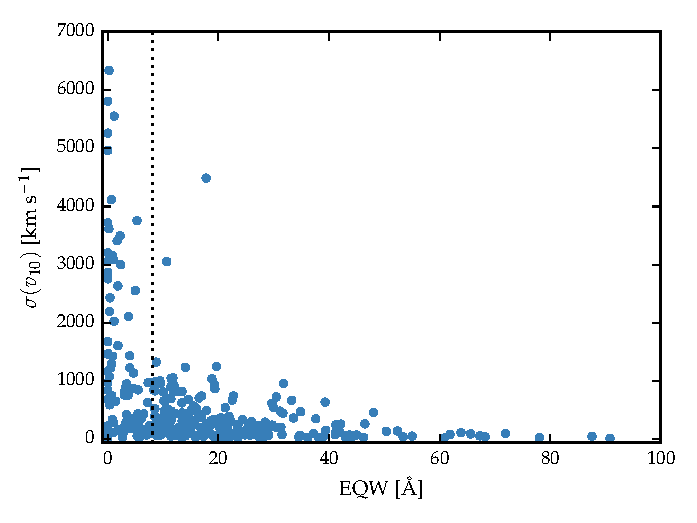
\includegraphics[width=0.8\textwidth]{figures/chapter04/eqw_cut.pdf} 
    \caption[{Uncertainty in $v_{10}$ as a function of the EQW, for [\ion{O}{III}].}]{Uncertainty in $v_{10}$ as a function of the EQW, for [\ion{O}{III}]. Uncertainties in $v_{10}$ are large to the left of the vertical line, at $8$\,\AA. These objects are ignored in our subsequent analysis of the [\ion{O}{III}] line shape.}     
    \label{fig:eqw_cut}
\end{figure}

In Figure~\ref{fig:eqw_cut} we show how the uncertainty in [\ion{O}{III}] $v_{10}$ depends on the EQW. 
As the strength of [\ion{O}{III}] decreases, the average uncertainty in $v_{10}$ increases.
When the [\ion{O}{III}] $\text{EQW} > 80$\,\AA, the mean uncertainty in $v_{10}$ is $50$\,\kms; this increases to $450$\,\kms\, when $10 < \text{EQW} < 20$\,\AA. 
As the EQW drops below $8$\,\AA, uncertainties in $v_{10}$ become very large (exceeding $1000$\,\kms\, in many objects). 
Clearly, the emission-line is too weak for its shape to be reliably measured in many of these objects. 
Therefore, when the [\ion{O}{III}] line properties (e.g. velocity-width, centroid) are analysed in later sections, objects with $\text{EQW} < 8$\,\AA\, will be excluded. 
This leaves $226$ quasars in the sample. 

\subsection{Reliability of systemic redshift estimates}
\label{sec:ch4_redshifts}

\begin{figure}
   \captionsetup[subfigure]{labelformat=empty}
    \centering
    \subfloat[\label{fig:redshift_comparison_a}]{}
    \subfloat[\label{fig:redshift_comparison_b}]{}
    \subfloat[\label{fig:redshift_comparison_c}]{}
    \subfloat[]{{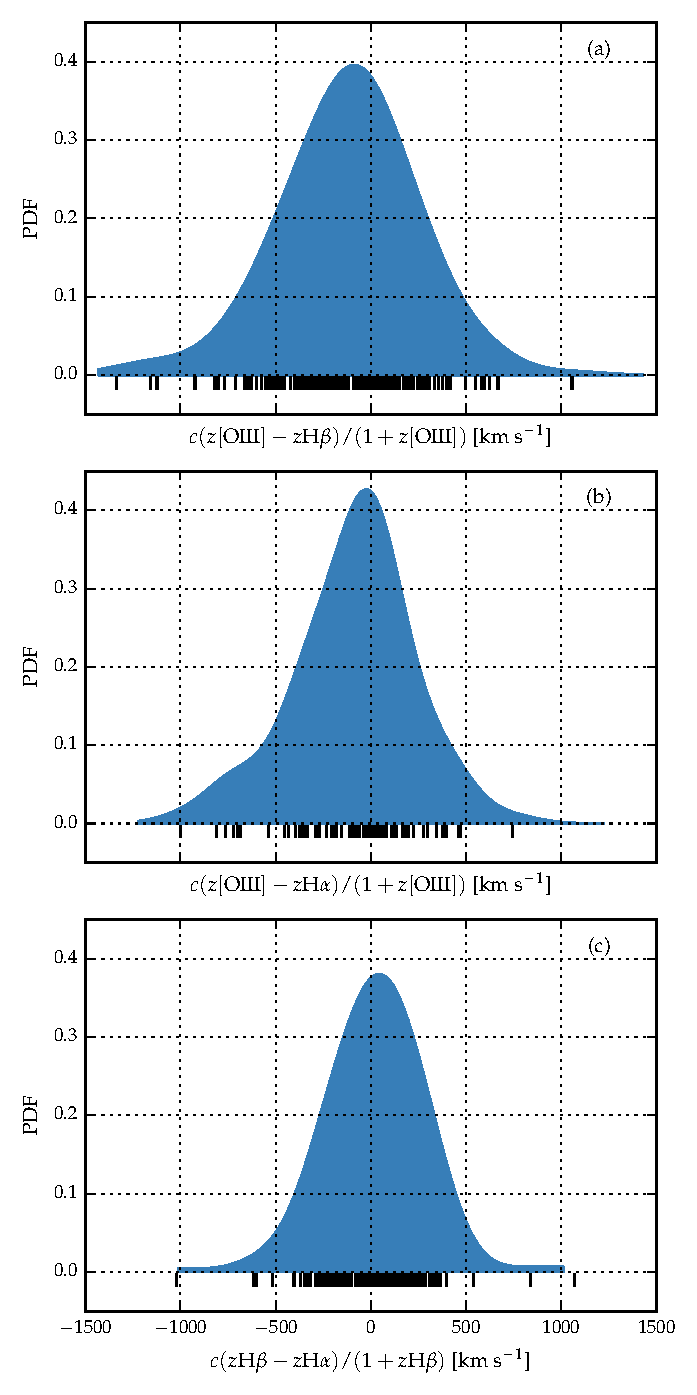
\includegraphics[width=0.8\linewidth]{figures/chapter04/redshift_comparison.pdf} }}
    \caption[{Comparison of systemic redshift estimates using [\ion{O}{III}], \hb and \hans.}]{Comparison of systemic redshift estimates using [\ion{O}{III}], \hb and \hans. The probability density distributions are generated using a Gaussian kernel density estimator with $170$, $120$ and $140$\,\kms\, kernel widths for (a), (b) and (c) respectively. The short black lines show the locations of the individual points.}       
    \label{fig:redshift_comparison}
\end{figure}

In this section, we compare systemic redshift estimates based on [\ion{O}{III}], \hb and \hans. 
The wavelength of each of these lines is measured at the peak of the emission and this measurement is made using the best-fitting parametric model. 
In the case of the Balmer lines, this model includes both broad and (if present) narrow emission features. 

We compare systemic redshift estimates based on [\ion{O}{III}] and \hb (Figure~\ref{fig:redshift_comparison_a}), [\ion{O}{III}] and \ha (Figure~\ref{fig:redshift_comparison_b}) and \hb and \ha (Figure~\ref{fig:redshift_comparison_c}). 
We generate probability density distributions using a Gaussian kernel density estimator.
The kernel width, which is optimised using leave-one-out cross-validation, is $170$, $120$ and $140$\,\kms\, in Figures~\ref{fig:redshift_comparison_a}, \ref{fig:redshift_comparison_b} and \ref{fig:redshift_comparison_c} respectively. 

There are $182$, $85$ and $162$ objects being compared in Figures~\ref{fig:redshift_comparison_a}, \ref{fig:redshift_comparison_b} and \ref{fig:redshift_comparison_c} respectively. 
We have excluded [\ion{O}{III}], \hb and \ha measurements when the uncertainties on the peak velocities exceed $200$, $300$ and $200$\,\kms\, respectively. 
We also exclude [\ion{O}{III}] measurements from 16 objects with very broad, blueshifted [\ion{O}{III}] emission that is strongly blended with the red wing of \hb (these objects are discussed in Section~\ref{sec:extreme_oiii}).

The scatter between the different redshift estimates ($360$, $280$, and $230$\,\kms\, in Figures~\ref{fig:redshift_comparison_a}, \ref{fig:redshift_comparison_b} and \ref{fig:redshift_comparison_c} respectively) is consistent with previous studies of redshift uncertainties from broad emission-lines \citep[e.g.][]{shen16b}. 
The systematic offset between the \ha and \hb estimates is effectively zero. 
However, the [\ion{O}{III}] redshifts appear to be systematically offset in comparison to both \ha and \hbns, in the sense that [\ion{O}{III}] is blueshifted in the rest-frame of the Balmer lines. 
This effect is strongest when [\ion{O}{III}] is compared to \hbns, in which case [\ion{O}{III}] is shifted by $\sim100$\,\kms\, to the blue.

\citet{hewett10} found that [\ion{O}{III}] was blueshifted by $\sim45$\,\kms\, relative to a rest-frame defined using photospheric \ion{Ca}{II}\ll$3935$,$3970$ absorption in the host galaxies of $z<0.4$ SDSS AGN and that [\ion{O}{III}] is increasingly blue-asymmetric at higher luminosities. 
Therefore, the $100$\,\kms offset we measure is consistent with \citet{hewett10} once the very different luminosities of the two samples are accounted for. 

\section{Results}

\subsection{Strength and kinematics of [\ion{O}{III}]}
\label{sec:ch4-basicresults}

\begin{figure}
    \captionsetup[subfigure]{labelformat=empty}
    \centering
    \subfloat[\label{fig:parameter_hists_a}]{}
    \subfloat[\label{fig:parameter_hists_b}]{}
    \subfloat[\label{fig:parameter_hists_c}]{}
    \subfloat[]{{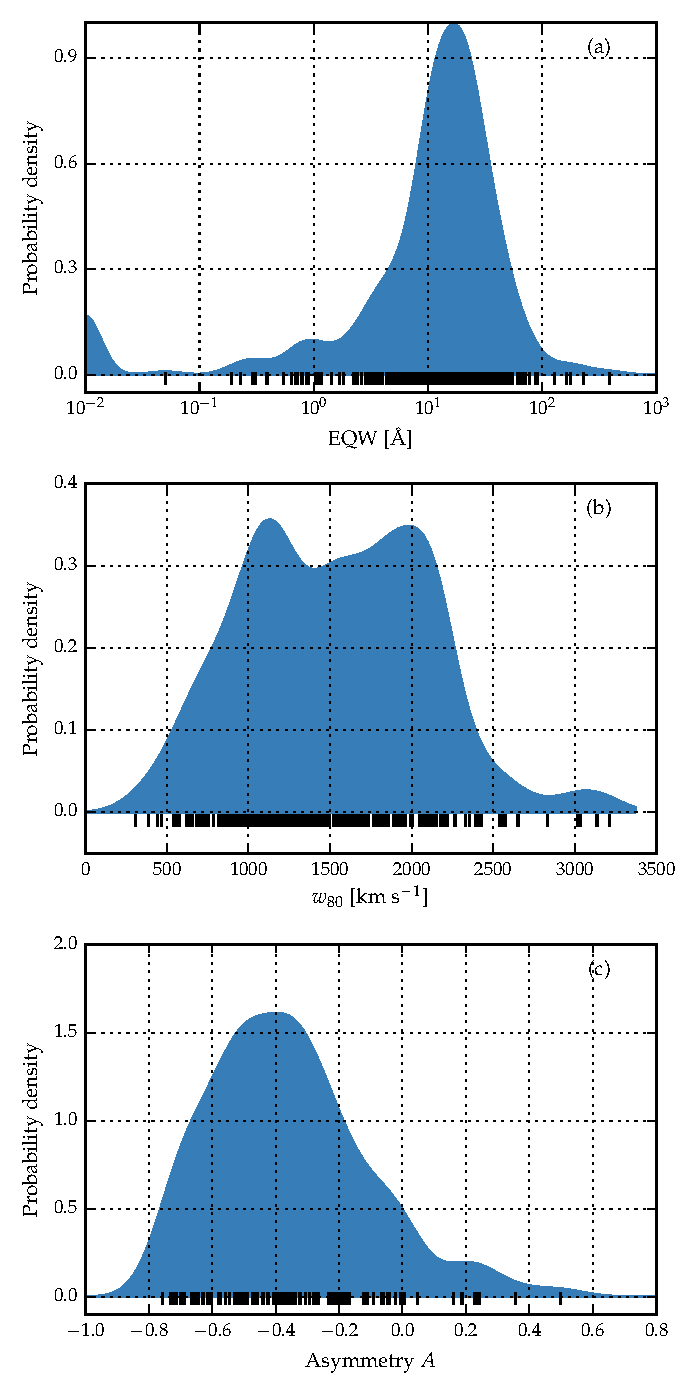
\includegraphics[width=0.8\columnwidth]{figures/chapter04/parameter_hists.pdf} }}
    \caption[{Probability density distributions of the [\ion{O}{III}] parameters EQW, $w_{80}$ and asymmetry $A$.}]{Probability density distributions of the [\ion{O}{III}] parameters EQW (a), $w_{80}$ (b) and asymmetry $A$ (c), generated using Gaussian kernel density estimation. The $1200$\,\kms\, upper limit on the velocity-width of the Gaussian functions used to model [\ion{O}{III}] is responsible for the peak at $1200$\,\kms\, in (b).}     
    \label{fig:parameter_hists}
\end{figure}

In our sample of $330$ quasars we observe a significant diversity in [\ion{O}{III}] emission properties. 

The probability density distribution of the [\ion{O}{III}] EQW is shown in Figure~\ref{fig:parameter_hists_a}. 
The median of the distribution is $14$\,\AA\, and the $68$ percentile range is $3$ to $30$\,\AA.
The maximum EQW is $391$\,\AA.  
In $10$ per cent of the sample [\ion{O}{III}] is very weak, with $\text{EQW} < 1$\,\AA.  

The median of the line-width (characterized by $w_{80}$ and shown in Figure~\ref{fig:parameter_hists_b}) is $1540$\,\kms\, and the $68$ percentile range is $950$ to $2100$\,\kms, with a minimum of $300$\,\kms\, and a maximum of $3200$\,\kms.

The [\ion{O}{III}] asymmetry is shown in Figure~\ref{fig:parameter_hists_c}. 
In $40$ per cent of the sample [\ion{O}{III}] is fit with a single Gaussian. 
The asymmetry is zero in this model and so these objects are excluded. 
For the [\ion{O}{III}] emission-lines modelled with two Gaussians, [\ion{O}{III}] is blue-asymmetric in $90$ per cent.
The median asymmetry is $-0.37$ and the $68$ percentile range is $-0.61$ to $-0.12$.

Blue-asymmetric structure and high-velocity gas is generally associated with outflows. 
Our results suggests that NLR outflows are prevalent in this sample of luminous quasars. 

We also find weak correlations between these three [\ion{O}{III}] parameters. 
The EQW is anti-correlated with both the line-width and asymmetry: as the [\ion{O}{III}] emission gets weaker it gets broader and more blue-asymmetric \citep[e.g.][]{shen14}.  

\subsection{Luminosity-dependence of [\ion{O}{III}] properties}
\label{sec:ch4-lumdependence}

In this section, we compare our sample of luminous $2 \lesssim z \lesssim 4$ quasars to a sample of $z\lesssim1$ SDSS quasars in order to investigate the luminosity and redshift dependence of key [\ion{O}{III}] parameters. 
We use $20\,663$ quasars with [\ion{O}{III}] measurements from the \citet{shen11} catalogue. 
The median redshift of these objects is $0.55$ and the median bolometric luminosity is $10^{45.5}$\,\ergs.

\begin{figure}[t!]
\centering 
    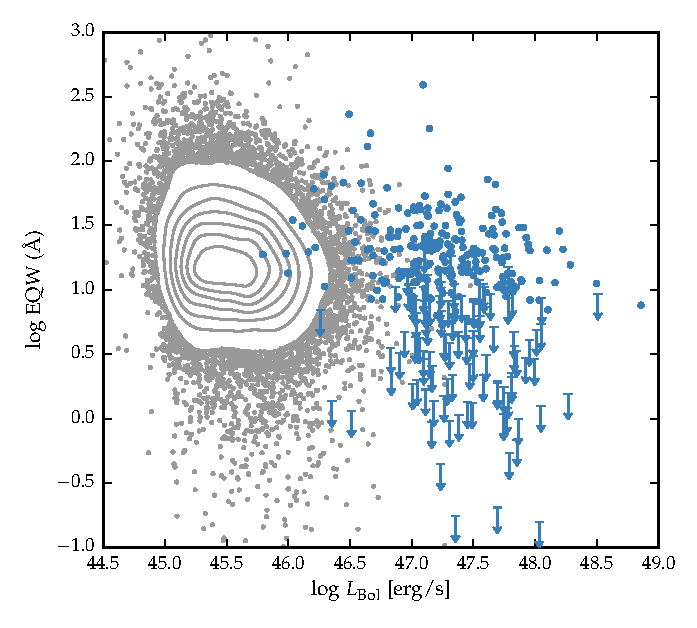
\includegraphics[width=\columnwidth]{figures/chapter04/eqw_lum.pdf} 
    \caption[{The [\ion{O}{III}] EQW as a function of the quasar bolometric luminosity.}]{The [\ion{O}{III}] EQW as a function of the quasar bolometric luminosity for the sample of luminous quasars presented in this chapter and the $z\lesssim1$ SDSS sample. An upper limit at $\text{EQW}=1$\,\AA\, indicates points with $\text{EQW} < 1$\,\AA. The solid line shows the median [\ion{O}{III}] EQW as a function of luminosity and the dashed lines show the $1$-$\sigma$ standard error on the median. The average EQW decreases from $17$ to $12$\,\AA\, over the luminosity range considered. At the same time, the fraction of quasars with very weak [\ion{O}{III}] ($\text{EQW} < 1$\,\AA) is ten times higher in the luminous quasar sample.}     
    \label{fig:eqw_lum}
\end{figure}

In Figure~\ref{fig:eqw_lum} we show the [\ion{O}{III}] EQW as a function of the quasar bolometric luminosity. 
Bolometric luminosities are estimated from monochromatic continuum luminosities at $5100$\,\AA, using the correction factor given by \citet{richards06}. 
Considering only the objects for which [\ion{O}{III}] is detected with $\text{EQW} > 1$\,\AA, we observe a decrease in the [\ion{O}{III}] EQW as the luminosity increases (from $17$\,\AA\, at $L_{\text{Bol}}=10^{45.25}$\,\ergs\, to $12$\,\AA\, at $L_{\text{Bol}}=10^{47.75}$\,\ergs). 
Given the luminosity spans a full $2.5$\,dex, the decrease in the [\ion{O}{III}] EQW ($30$ per cent) is very modest.
However, [\ion{O}{III}] $\text{EQW} < 1$\,\AA\, in $10$ per cent of the luminous quasars, compared to just one per cent of the $z \lesssim 1$ SDSS sample.
This is explored further in Section~\ref{sec:ch4-civtrends}.  

Many authors have reported the [\ion{O}{III}] EQW to decrease with quasar luminosity \citep[e.g.][]{brotherton96,sulentic04,baskin05b,zhang11,stern12}.
The origin of this correlation - known as the [\ion{O}{III}] Baldwin effect \citep[e.g.][]{baldwin77} - has not been demonstrated conclusively. 
The size of the NLR (and hence the [\ion{O}{III}] luminosity) is predicted to scale with the square root of the luminosity of the source of ionising photons \citep[e.g.][]{netzer90} and low-luminosity Seyfert galaxies appear to obey this relationship \citep[e.g.][]{bennert02}. 
Extrapolating this relationship to high luminosity quasars leads to the prediction of NLRs with galactic dimensions.
Under these conditions, the size of the NLR will be limited by the density and ionisation state in the NLR. 
In other words, the NLR can't continue to grow beyond the radius at which there is no longer gas available to be ionised and the luminosity of the NLR will saturate \citep[e.g.][]{hainline13,hainline14}. 

\begin{figure}[t!]
    \centering
    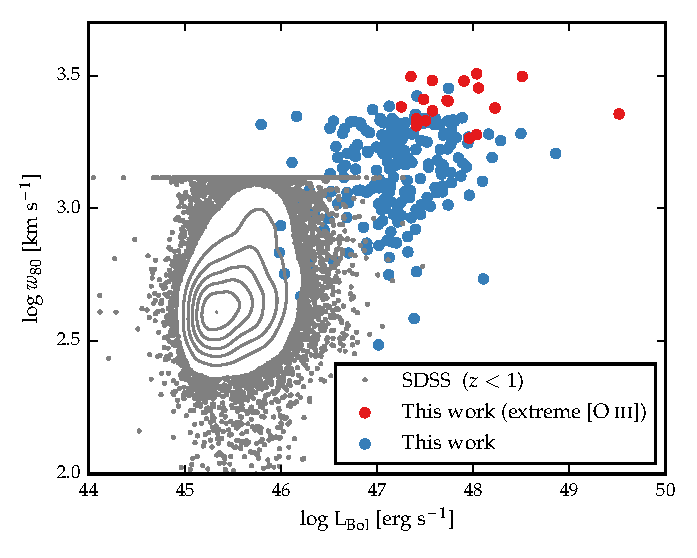
\includegraphics[width=\columnwidth]{figures/chapter04/lum_w80.pdf} 
    \caption[{[\ion{O}{III}] velocity-width $w_{80}$ as a function of quasar bolometric luminosity.}]{[\ion{O}{III}] velocity-width $w_{80}$ as a function of quasar bolometric luminosity. Objects with extreme [\ion{O}{III}] profiles (Section~\ref{sec:extreme_oiii}) are shown in red. The grey dots show $z\lesssim1$ SDSS quasars. The FWHM measurements given by \citet{shen11} have been converted into equivalent $w_{80}$ values by assuming $w_{80} \simeq \text{FWHM} / 0.919$. The build-up of points at $w_{80}=1300$\,\kms\, is caused by the upper-limit $1200$\,\kms\, imposed by \citet{shen11} on the [\ion{O}{III}] FWHM. The typical [\ion{O}{III}] velocity-width increases from $440$\,\kms\, at $\log L_{\text{Bol}}=45.5$\,\ergs\, to $1850$\,\kms\, at $\log L_{\text{Bol}}=48$\,\ergs.} 
    \label{fig:lum_w80}
\end{figure}

In Figure~\ref{fig:lum_w80} we show that the [\ion{O}{III}] velocity-width is also strongly correlated with the quasar bolometric luminosity.
The typical [\ion{O}{III}] velocity-width increases from $440$\,\kms\, at $\log L_{\text{Bol}}=45.5$\,\ergs\, to $1850$\,\kms\, at $\log L_{\text{Bol}}=48$\,\ergs.  
This demonstrates that the highest velocity outflows are associated with the most luminous AGN which suggests that the outflows are driven by radiative forces. 

Considering only objects in a narrow luminosity range ($47 < \log L_{\text{Bol}} < 47.5$\,\ergs) we observe no correlations between the redshift and either the [\ion{O}{III}] velocity-width or EQW.   
The lack of any evolution in typical [\ion{O}{III}] properties between $z=0$ and $z=1.5$ has previously been reported \citep[e.g.][]{harrison16}; our sample demonstrates that the [\ion{O}{III}] properties do not evolve from $z=1.5$ all the way to $z=4$. 

\subsection{EV$1$ trends in high-redshift quasars}

\begin{figure}[t!]
\centering 
    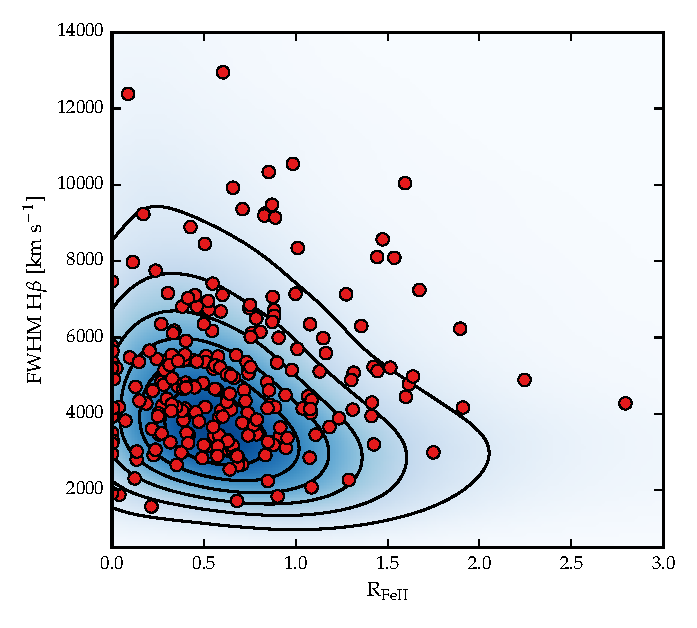
\includegraphics[width=\columnwidth]{figures/chapter04/ev1_lowz.pdf} 
    \caption[{The distribution of objects in the EV$1$ parameter space.}]{The distribution of objects in the EV$1$ parameter space. The distribution of luminous quasars (shown using circles) is similar to the distribution of $z \lesssim 1$ SDSS quasars (shown using contours), with the displacement to higher \hb FWHM indicative of higher BH masses in the luminous sample.}      
    \label{fig:ev1_lowz}
\end{figure}

The FWHM of the broad \hb emission-line, the strength of [\ion{O}{III}] and the relative strengths of optical \ion{Fe}{II} and \hb have been identified as the features responsible for the largest variance in the spectra of AGN and form part of EV$1$ \citep{boroson92}.   
In Figure~\ref{fig:ev1_lowz} we show the [\ion{O}{III}] EQW as a function of the \hb FWHM and the optical \ion{Fe}{II} strength. 
The optical \ion{Fe}{II} strength is defined as the ratio of the \ion{Fe}{II} and \hb EQW, where the \ion{Fe}{II} EQW is measured between $4434$ and $4684$\,\AA.
There are $231$ objects in our sample with spectra that include \hbns, [\ion{O}{III}], and at least $150$\,\AA\, of the $4434$-$4684$\,\AA\, \ion{Fe}{II} region.  
For comparison, $z\lesssim1$ SDSS quasars are also shown in Figure~\ref{fig:ev1_lowz}. 
 
In our sample, the EV$1$ parameters follow similar correlations to what is observed at low-redshift.
In particular, we observe a strong anti-correlation between the [\ion{O}{III}] and \ion{Fe}{II} EQW.  
The \hb FWHM are displaced to higher values, which is consistent with the high-redshift, high-luminosity sample having larger BH masses. 
Thus, with a much bigger sample, we confirm earlier results suggesting that the same EV$1$ correlations exist in high-redshift quasars \citep[e.g.][]{netzer04,sulentic04,sulentic06,runnoe13,shen16a}.
This suggests that similar underlying physical processes govern the spectral properties of AGN and quasars over a wide range of redshifts and luminosities. 

\subsection{Connections with \ion{C}{IV} emission properties}
\label{sec:ch4-civtrends}

\begin{figure}[t!]
\centering 
    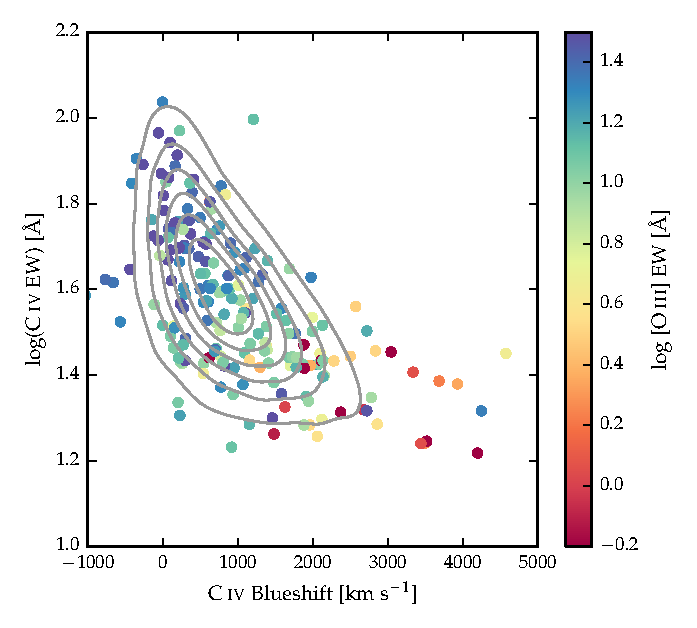
\includegraphics[width=0.9\textwidth]{figures/chapter04/ev1.pdf} 
    \caption[{Parameter space of \ion{C}{IV} blueshift and EQW.}]{Parameter space of \ion{C}{IV} blueshift and EQW. Our sample is shown with the coloured circles, and quasars from the full SDSS catalogue are shown with grey contours. The [\ion{O}{III}] EQW varies systematically across the \ion{C}{IV} blueshift-EQW parameter space. In the small \ion{C}{IV} blueshift, high EQW region the mean [\ion{O}{III}] EQW is $47$\,\AA; this drops dramatically to $6$\AA\, in the large \ion{C}{IV} blueshift, low EQW region.}      
    \label{fig:ev1}
\end{figure}

Like the EV$1$ parameter space, the \ion{C}{IV} blueshift and EQW are diagnostics that similarly span the diversity of broad emission-line properties in high redshift quasars \citep{sulentic07,richards11}. 
In Figure~\ref{fig:ev1} we show the [\ion{O}{III}] EQW as a function of the \ion{C}{IV} blueshift and EQW.
When [\ion{O}{III}] is strong, the \ion{C}{IV} blueshift is measured relative to the [\ion{O}{III}] peak. 
Otherwise, the \ion{C}{IV} blueshift is measured relative to \hb or \hans.  
In Section~\ref{sec:ch4_redshifts} we found that redshifts measured from [\ion{O}{III}], \hb and \ha are consistent to within $\sim300$\,\kms, which is small in comparison to the dynamic range in \ion{C}{IV} blueshifts we see in Figure~\ref{fig:ev1}.
Also shown are the \ion{C}{IV} line parameters of $32\,157$ SDSS DR$7$ quasars at redshifts $1.6 < z < 3.0$. 
For this sample, systemic redshifts are taken from Allen \& Hewett (2017, in preparation). 

The [\ion{O}{III}] EQW decreases systematically from the small \ion{C}{IV} blueshift, large EQW region of the parameter space to the large \ion{C}{IV} blueshift, small EQW region.
In the top left of the distribution (\ion{C}{IV} blueshift $<1000$\,\kms, $\text{EQW} > 60$\,\AA) the mean [\ion{O}{III}] EQW is $47$\,\AA; this drops dramatically to $6$\AA\, in the bottom right (\ion{C}{IV} blueshift $>2000$\,\kms, $\text{EQW} < 30$\,\AA). 

Qualitatively, the distribution of objects in the \hb FWHM - \ion{Fe}{II} strength EV$1$ parameter space (Figure~\ref{fig:ev1_lowz}) is very similar to the distribution of objects in the \ion{C}{IV} blueshift-EQW parameter space (Figure~\ref{fig:ev1}).
In Figure~\ref{fig:line_comparison_ha} we showed that objects with large \ion{C}{IV} blueshifts also have narrow \ha emission-lines.
However, the converse is not true: many of the objects with narrow \ha emission-lines also have small \ion{C}{IV} blueshifts. 
In contrast, Figure~\ref{fig:ev1} demonstrates that the [\ion{O}{III}] EQW provides a less degenerate mapping between the EV$1$ and \ion{C}{IV} parameter spaces.

\begin{figure}
    \centering
    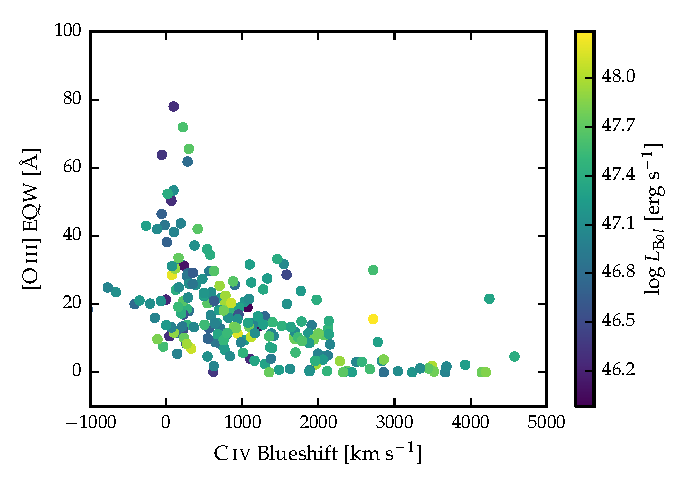
\includegraphics[width=\columnwidth]{figures/chapter04/civ_blueshift_oiii_eqw.pdf} 
    \caption[{[\ion{O}{III}] EQW as a function of the \ion{C}{IV} blueshift.}]{[\ion{O}{III}] EQW as a function of the \ion{C}{IV} blueshift. The [\ion{O}{III}] EQW is strongly anti-correlated with the \ion{C}{IV} blueshift. On the other hand, no strong luminosity-dependent trends (indicated by the colours of the points) are evident.}     
    \label{fig:civ_blueshift_oiii_eqw}
\end{figure}

A different projection of the same data is shown in Figure~\ref{fig:civ_blueshift_oiii_eqw}, which shows the [\ion{O}{III}] EQW as a function of the \ion{C}{IV} blueshift.  
The luminosity of the quasars is indicated by the colour of the points. 
Both the [\ion{O}{III}] EQW and the \ion{C}{IV} blueshift are known to depend on the quasar luminosity. 
However, Figure~\ref{fig:civ_blueshift_oiii_eqw} demonstrates that the strong correlation between the \ion{C}{IV} blueshift and [\ion{O}{III}] EQW is clearly not being driven by the mutual dependence of these parameters on the luminosity. 

Blueshifted \ion{C}{IV} emission is thought to arise in a high-velocity accretion disc wind.
The strong anti-correlation between the \ion{C}{IV} blueshift and the [\ion{O}{III}] EQW suggests that these outflows are having a dramatic impact on gas extended over kilo-parsec scales in the NLR.
Dynamical time-scales for the impact of fast moving outflows even on large NLRs are very short: it would take $10^6$ years for an outflow travelling at $3000$\,\kms\, to reach $3$\,kilo-parsec. 
Lifetimes of luminous quasars at these redshifts may be $10^7$ years \citep[e.g.][]{martini01}. 
Therefore, if the BLR outflows can break out into the interstellar medium of the host-galaxy, the NLR can be cleared on a relatively short time-scale.
One possibility is that the BLR winds collide with the interstellar medium and shock and accelerate it to produce a galaxy-wide wind \citep[e.g.][]{king11,faucher12}. 
\ion{C}{IV} blueshifts are generally weaker in lower-luminosity quasars. 
Therefore, this picture also explains our finding that objects with very weak [\ion{O}{III}] ($\text{EQW} < 1$\,\AA) are ten times rarer in $z \lesssim 1$ SDSS quasars than in our sample of luminous quasars.   

\subsection{A link between BLR and NLR outflows}

\begin{figure}[t!]
    \centering
    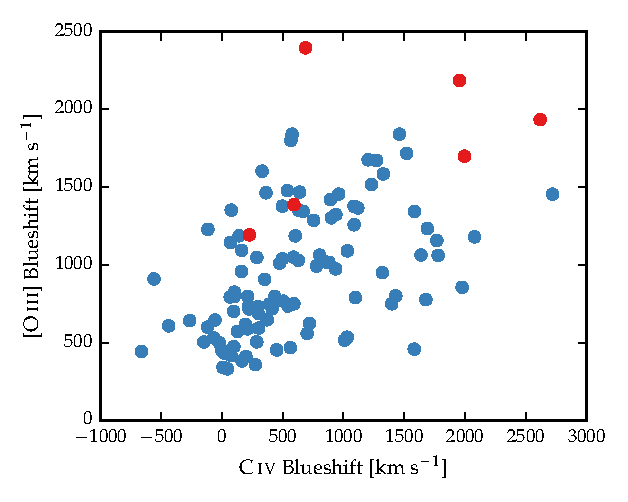
\includegraphics[width=\linewidth]{figures/chapter04/civ_blueshift_oiii_blueshift.pdf} 
    \caption[{Relationship between the \ion{C}{IV} and [\ion{O}{III}] blueshifts.}]{Relationship between the \ion{C}{IV} ($v_{50}$(\ion{C}{IV}) - $v_{\text{peak}}$([\ion{O}{III}])) and [\ion{O}{III}] ($v_{10}$([\ion{O}{III}]) - $v_{\text{peak}}$([\ion{O}{III}])) blueshift. The \ion{C}{IV} and [\ion{O}{III}] blueshifts are correlated with $\rho_{\text{S}}=0.46$. This correlation is independent of the luminosity (indicated by the colour of the points). }
    \label{fig:oiii_civ_blueshifts}
\end{figure}

\begin{figure}
\captionsetup[subfigure]{labelformat=empty}
\centering 
    \subfloat[\label{fig:oiii_civ_blueshifts_a}]{}
    \subfloat[\label{fig:oiii_civ_blueshifts_b}]{}
    \subfloat[]{{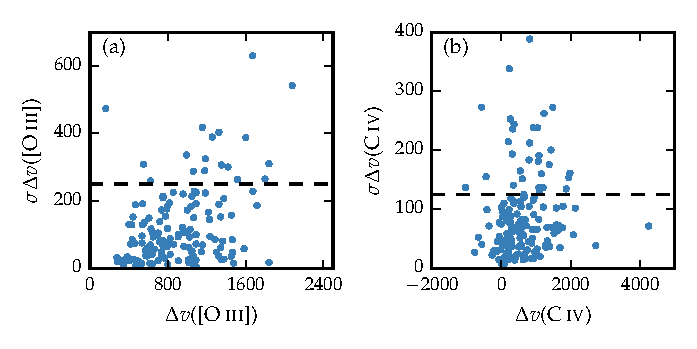
\includegraphics[width=\linewidth]{figures/chapter04/civ_blueshift_oiii_blueshift_flagged.pdf} }}
    \caption[{Objects excluded from in Figure~\ref{fig:oiii_civ_blueshifts}.}]{Objects with errors on the [\ion{O}{III}] and \ion{C}{IV} blueshifts exceeding $250$ or $125$\,\kms\, respectively are excluded from Figure~\ref{fig:oiii_civ_blueshifts}. The [\ion{O}{III}] and \ion{C}{IV} blueshifts of these objects, which lie above the dashed lines in (a) and (b), are similar to the main sample, meaning our results should not be biased by their exclusion.}
    \label{fig:oiii_civ_blueshifts_flagged}
\end{figure}

In Figure~\ref{fig:oiii_civ_blueshifts} we show that the [\ion{O}{III}] blueshift is correlated with the \ion{C}{IV} blueshift.
The Spearman correlation coefficient, $\rho_{\text{S}}$, is $0.46$, with p-value $=6\times10^{-7}$. 
This shows that high-velocity winds in the NLR are preferentially seen when strong winds are being driven in the vicinity of the central engine. 
As we demonstrate in Figure~\ref{fig:oiii_civ_blueshifts}, this correlation is not driven by the luminosity. 
Although we lack direct spatial information, this correlation suggests a connection between gas kinematics on sub-parsec and kilo-parsec scales. 

The [\ion{O}{III}] blueshift is defined as $v_{10}$([\ion{O}{III}]) - $v_{\text{peak}}$([\ion{O}{III}]) and the \ion{C}{IV} blueshift is defined as $v_{50}$(\ion{C}{IV}) - $v_{\text{peak}}$([\ion{O}{III}]).
We considered a number of alternative approaches to parametrising both the [\ion{O}{III}] line shape and the systemic redshift. 
Very similar trends are observed when the [\ion{O}{III}] line shape is parametrised using $v_{25} - v_{\text{peak}}$, $v_{50} - v_{\text{peak}}$, $w_{80} = v_{90} - v_{10}$, or the asymmetry $A$.
The same trend is also observed when the systemic redshift is defined using the peak of the \hb emission. 

In the previous section, we saw how [\ion{O}{III}] is very weak in quasars with \ion{C}{IV} blueshifts exceeding $\sim2000$\,\kms. 
The [\ion{O}{III}] blueshift cannot be reliably measured if the emission-line $\text{EQW} \lesssim 8$ (Section~\ref{sec:ch4-loweqw}) and so this limits the dynamic range of \ion{C}{IV} blueshifts probed in Figure~\ref{fig:oiii_civ_blueshifts}. 
We do not show objects for which the errors on the [\ion{O}{III}] and \ion{C}{IV} blueshifts exceed $250$ or $125$\,\kms\, respectively. 
The [\ion{O}{III}] and \ion{C}{IV} blueshifts of these objects, shown in Figures~\ref{fig:oiii_civ_blueshifts_a} and \ref{fig:oiii_civ_blueshifts_b}, are similar to the main sample, meaning our results should not be biased by their exclusion.  
We also remove the objects with extreme [\ion{O}{III}] emission (Section~\ref{sec:extreme_oiii}), because the systemic redshift determined from the peak of the [\ion{O}{III}] emission is strongly biased in these objects. 

\citet{shen14} showed how the [\ion{O}{III}] EQW decreases as the optical \ion{Fe}{II} strength (which is related to the Eddington ratio) or luminosity increase. 
However, the amplitude of the systemic, core [\ion{O}{III}] emission decreases faster than the wing component.
A by-product of this effect is that the overall [\ion{O}{III}] profile becomes broader and more blueshifted, as the broad wing component becomes relatively more prominent.
If the anti-correlation between the [\ion{O}{III}] EQW and \ion{C}{IV} blueshift is primarily being driven by a reduction in the flux of the core component (as a stable NLR is removed by the outflowing material), this would lead to a correlation between the [\ion{O}{III}] blueshift and \ion{C}{IV} blueshift similar to the one seen in Figure~\ref{fig:oiii_civ_blueshifts}. 
This effect could also explain the anti-correlation between the [\ion{O}{III}] EQW and blue-asymmetry / velocity-width we reported in Section~\ref{sec:ch4-basicresults}. 

\subsection{The BAL parent population}

Classical high-ionization BAL (HiBAL) quasars are likely to be radiating with relatively high $L/L_{\text{Edd}}$ \citep[e.g.][]{zhang14}. 
We therefore propose that the subset of the quasar population that exhibits large \ion{C}{IV}-emission blueshifts may be directly related to the HiBAL quasar population \---\ perhaps even the `parent' population \citep{richards06conf}. 

To test this hypothesis, we selected $18$ \ion{C}{IV} BAL quasars from our catalogue which have near-infrared spectra including \hbns. 
Using the same method described in Section~\ref{sec:hahbcomparison}, we constructed a median composite spectrum from this sample. 
For comparison, we also constructed composite spectra for quasars with modest and large \ion{C}{IV} blueshifts. 
The results are shown in Figure~\ref{fig:bal_composite}. 
We find that [\ion{O}{III}] is very weak in the BAL quasars and that the median [\ion{O}{III}] emission profiles in the BAL quasars and non-BAL quasars with large \ion{C}{IV} blueshifts are very similar \citep[e.g.][]{yuan03}.
On the other hand, \hb is narrower in BAL quasars than in non-BAL quasars (with or without large \ion{C}{IV} blueshifts).
One possibility is that, while the [\ion{O}{III}] emission is relatively isotropic, the \hb FWHM has some dependence on the orientation of the BLR \citep[e.g.][]{shen14}.
In this scenario, the narrow \hb emission suggests that BAL quasars are preferentially observed in relatively face-on orientations. 

\begin{figure}[t!]
    \centering
    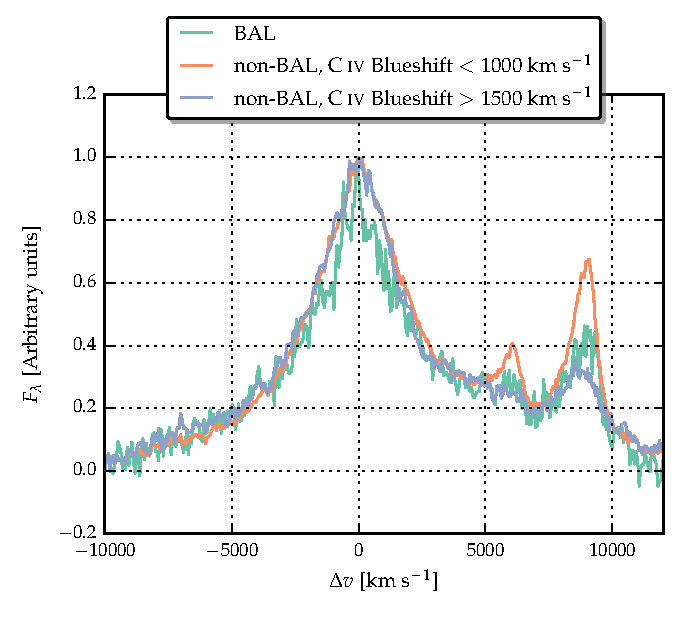
\includegraphics[width=0.8\linewidth]{figures/chapter04/bal_composite.pdf}
    \caption[{Composite spectra of the \hbns/[\ion{O}{III}] region for BAL and non-BAL quasars.}]{Composite spectra of the \hbns/[\ion{O}{III}] region made of BAL quasars, non-BAL quasars with \ion{C}{IV} blueshifts below $1000$\,\kms, and non-BAL quasars with \ion{C}{IV} blueshifts above $1500$\,\kms. [\ion{O}{III}] is similar in BAL quasars and non-BAL quasars with large \ion{C}{IV} blueshifts, whereas \hb is narrower in the BAL quasars.}
    \label{fig:bal_composite}
\end{figure}

\subsection{Extreme [\ion{O}{III}] profiles}
\label{sec:extreme_oiii}

\begin{figure}
    \centering
    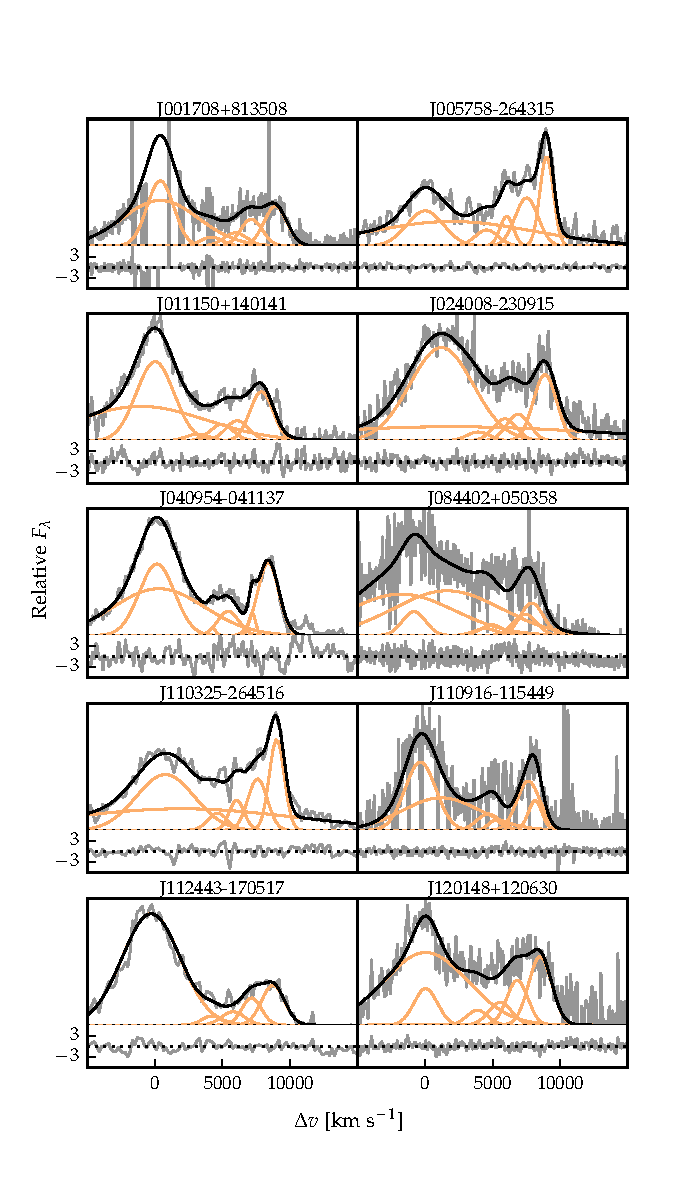
\includegraphics[width=\columnwidth]{figures/chapter04/example_spectrum_grid_extreme_oiii_1.pdf} 
    \caption[{Model fits to the \hbns/[\ion{O}{III}] emission in $18$ quasars with extreme [\ion{O}{III}] emission profiles.}]{Model fits to the continuum- and \ion{Fe}{II}-subtracted \hbns/[\ion{O}{III}] emission in $18$ quasars with extreme [\ion{O}{III}] emission profiles. The data is shown in grey, the best-fitting model in black, and the individual model components in orange. The peak of the [\ion{O}{III}] emission is used to set the redshift, and $\Delta{v}$ is the velocity shift from the rest-frame transition wavelength of \hbns. Below each spectrum we plot the data- minus-model residuals, scaled by the errors on the fluxes.}     
    \label{fig:example_spectrum_grid_extreme_oiii}
\end{figure}

\begin{figure}[t!]
\ContinuedFloat
    \centering
    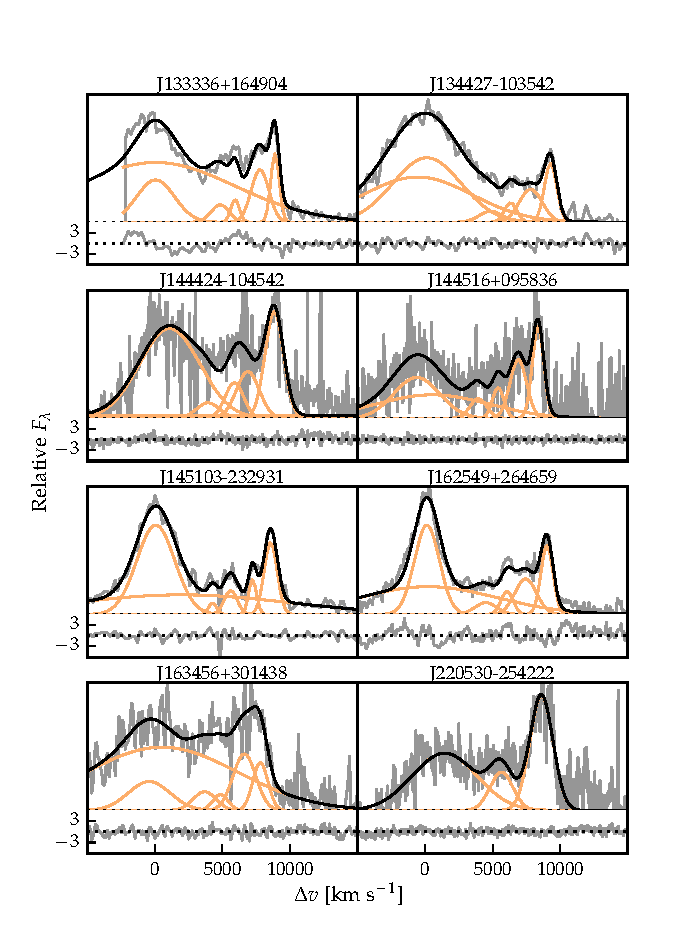
\includegraphics[width=\columnwidth]{figures/chapter04/example_spectrum_grid_extreme_oiii_2.pdf} 
    \caption[]{Continued.}     
\end{figure}

Figure~\ref{fig:example_spectrum_grid_extreme_oiii} shows the spectra of $18$ objects which we visually identified as having [\ion{O}{III}] emission profiles with similar characteristics to four extremely dust-reddened quasars at $z\sim2$ recently identified by \citet{zakamska16}. 
The extreme nature of the [\ion{O}{III}] emission in their sample of red quasars led \citet{zakamska16} to propose that these objects are being observed in the process of expelling the gas in their host-galaxies and transitioning from a dust-obscured, star-burst phase to a luminous, blue quasar \citep[e.g.][]{sanders88}.

The [\ion{O}{III}] emission in the $18$ objects in our sample is very broad ($1800 \lesssim w_{80} \lesssim 3200$\,\kms; Figure~\ref{fig:lum_w80}). 
In many of these objects the systemic, core component of [\ion{O}{III}] is not detected.
The [\ion{O}{III}] doublet is blended together, and is also heavily blended with the red wing of the \hb emission. 
The \ion{Fe}{II} emission may also be significant in this region of the spectrum. 

\begin{figure}
\centering 
    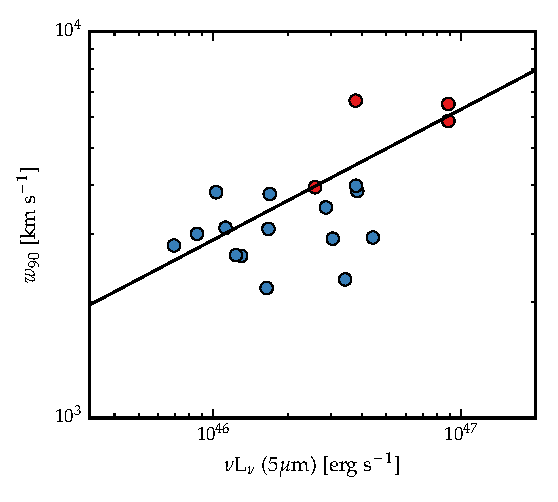
\includegraphics[width=0.8\textwidth]{figures/chapter04/fivemicron_w90.pdf} 
    \caption[{Velocity-widths and rest-frame $5$\,$\mu$m luminosities of the $18$ quasars in our sample with extreme [\ion{O}{III}] emission profiles and the four dust-reddened quasars from \citet{zakamska16}.}]{Velocity-widths, $w_{90}$, and rest-frame $5$\,$\mu$m luminosities of the $18$ quasars in our sample with extreme [\ion{O}{III}] emission profiles and the four dust-reddened quasars from \citet{zakamska16}. Our sample falls on the width-luminosity relation derived by \citet{zakamska16}.}     
    \label{fig:fivemicron_w90}
\end{figure}

In Figure~\ref{fig:fivemicron_w90} we compare the velocity-widths and rest-frame $5$\,$\mu$m luminosities of the $18$ quasars in our sample with the four quasars from \citet{zakamska16}.
On average, the \citet{zakamska16} quasars have higher luminosities ($10^{46.7}$ versus $10^{46.3}$\ergs) and the [\ion{O}{III}] emission is broader ($5740$ versus $3120$\,\kms).
However, the [\ion{O}{III}] velocity-width and luminosity of the least extreme \citet{zakamska16} quasar has properties very similar to our sample, and our objects lie on top of the velocity-luminosity relation derived by \citet{zakamska16} (Figure~\ref{fig:fivemicron_w90}).

The [\ion{O}{III}] velocity-widths and luminosities of the $18$ quasars in Figure~\ref{fig:example_spectrum_grid_extreme_oiii} are very large, but are comparable to many other objects in our sample.
However, we find that of the six objects which fall within the footprint of the FIRST radio survey, four are radio-loud (three core-dominated and one lobe-dominated).
Given the fraction of radio-loud objects in our sample is $11$ per cent, the binomial probability of finding four radio-loud objects in a sample of six is $0.1$ per cent. 
Relativistic jets are known to accelerate gas to velocities of up to a few thousand \kms\, \citep[e.g.][]{nesvadba06,nesvadba08}, and this could be inducing the disturbed [\ion{O}{III}] gas kinematics of these objects. 

\section{Mass outflow rate and kinetic power}

The mass outflow rate and kinetic power of galaxy-wide outflows are important in order to understand the role played by quasars in the evolution of galaxies. 
In this section, we calculate the mass outflow rate ($\dot{M}$) and kinetic power ($P_{\text{K}}$) of the ionised outflows in our sample of luminous quasars, using the [\ion{O}{III}] emission as a gas tracer \citep[e.g.][]{harrison12,cano-diaz12,liu13,brusa15,carniani15,bischetti16,kakkad16}.  
By making reasonable assumptions for unknown quantities (including the geometry, spatial scale and density of the gas in the outflow) we can calculate order of magnitude estimates of the outflow properties.
Our calculations are based on the model of \citet{cano-diaz12}, and a comprehensive description of the assumptions in the model and their impact on the inferred outflow properties can be found in \citet{cano-diaz12} and \citet{kakkad16}. 

Following \citet{cano-diaz12}, the mass in the ionised outflow is given by 

\begingroup\makeatletter\def\f@size{11}\check@mathfonts
\begin{eqnarray}
M \simeq 5.33 \times 10^7 \left( \frac{C}{10^{[\text{O/H}] - [\text{O/H}]_\odot}} \right) \left( \frac{L([OIII])}{10^{44}\, \text{erg}\,\text{s}^{-1}}\right) \nonumber \\ \times \left\langle \frac{n_e}{10^3\, \text{cm}^{-3}} \right\rangle^{-1} \, M_\odot
\end{eqnarray}
\endgroup

\noindent where $L([OIII])$ is the luminosity of [\ion{O}{III}] emitted in the outflow (in units of $10^{44}$\,\ergs), $\langle n_e \rangle$ is the electron density in the outflowing gas (in units of $10^3$\,cm$^{-3}$), $10^{[\text{O/H}]}$ is the metallicity (in units of Solar metallicity), $C$ ($=\langle n_e \rangle ^2 / \langle n_e^2\rangle$) is the condensation factor (assumed to be $\simeq1$). 
Assuming a conical outflow with uniformly distributed clouds out to a radius $R$ with a constant outflow velocity, the mass outflow rate of the gas is given by: 

\begingroup\makeatletter\def\f@size{11}\check@mathfonts
\begin{eqnarray}
\dot{M} = 164 \left( \frac{R}{1\,\text{kpc}} \right)^{-1} \left( \frac{C}{10^{[\text{O/H}] - [\text{O/H}]_\odot}} \right) \left( \frac{L([OIII])}{10^{44}\, \text{erg}\,\text{s}^{-1}}\right) \nonumber \\ \times \left( \frac{v}{1000\,\text{km}\,\text{s}^{-1}}\right) \times \left\langle  \frac{n_e}{10^3\, \text{cm}^{-3}} \right\rangle^{-1} \, M_\odot \, \text{yr}^{-1}
\end{eqnarray}
\endgroup

\noindent where $v$ is the outflow velocity (in units of $1000$\,\kms).
The kinetic power of the outflow ($1/2\dot{M}v^2$) is given by: 

\begingroup\makeatletter\def\f@size{11}\check@mathfonts
\begin{eqnarray}
P_{\text{K}} = 5.17 \times 10^{43} \left( \frac{R}{1\,\text{kpc}} \right)^{-1} \left( \frac{C}{10^{[\text{O/H}] - [\text{O/H}]_\odot}} \right) \left( \frac{L([OIII])}{10^{44}\, \text{erg}\,\text{s}^{-1}}\right) \nonumber \\ \times \left( \frac{v}{1000\,\text{km}\,\text{s}^{-1}}\right)^3 \times \left\langle \frac{n_e}{10^3\, \text{cm}^{-3}} \right\rangle^{-1} \, \text{erg}\,\text{s}^{-1}
\end{eqnarray}
\endgroup

\noindent We assume that the maximum outflow velocity ($\simeq v_{5}$) is representative of the average outflow velocity, with the lower velocities due to projection effects \citep{cano-diaz12}.
We assume the outflowing gas is represented by the broader of the two Gaussian components in our [\ion{O}{III}] model, and use the luminosity of this component to estimate the luminosity of the outflowing gas. 
This is not possible when [\ion{O}{III}] is modelled with a single Gaussian, and so these objects are not considered. 
For the outflow radius we use $4$\,kilo-parsec.
This is broadly consistent with spatially resolved observations of quasars at similar redshifts and luminosities \citep[e.g.][]{cano-diaz12,carniani15,brusa16} and photo-ionisation estimates \citep[e.g.][]{zakamska16}. 

With these values, we calculate outflow rates which range from a few to $4000\,M_\odot\,\text{yr}^{-1}$. 
The mean for our sample is $560\,M_\odot\,\text{yr}^{-1}$. 
In terms of the kinetic power of the outflows, this corresponds to values from about $10^{41.8}$ to $10^{45.7}$\,\ergs, with mean $10^{44.7}$\,\ergs. 
The mean kinetic power corresponds to $\sim0.15$ per cent of the bolometric luminosity, and this reaches almost $1$ per cent in the most powerful outflows.  
However, if the ionised outflow is accompanied by a neutral/molecular outflow an order of magnitude more massive then the kinetic power is also likely to be an order of magnitude higher \citep{cano-diaz12}, i.e. about $1.5$ per cent of the bolometric luminosity for the mean kinetic power and $10$ per cent for the most powerful outflows. 
These outflow efficiencies are in same ballpark as recent AGN feedback models \citep[e.g.][]{zubovas12}, which predict a coupling efficiency between AGN-driven outflows and AGN power of $\sim5$ per cent.

\section[MFICA]{Mean field independent component analysis}

Blind source separation (BSS) techniques can be used to find a set of basis vectors from a set of spectra. 
An individual spectrum can then be represented as a linear combination of the basis vectors with a corresponding set of weights.  
Principal component analysis (PCA) is one example of a BSS technique that has been applied extensively to analyse astronomical spectra \citep[e.g.][]{mittaz90,francis92,yip04}. 
However, in general it is not possible to physically interpret the individual PCA components. 
Mean field independent component analysis (MFICA) is more powerful class of BSS technique that works by finding a basis of independent components to represent the data.  
\citet{allen13} used this technique to analyse the SDSS spectra of emission-line galaxies and demonstrated its effectiveness in identifying distinct emission sources in the spectra. 

In this section, we use a set of ten MFICA-derived spectral components to reconstruct the rest-frame optical spectra of luminous quasars.
The MFICA components have been derived from a large sample of $z \lesssim 1$ SDSS spectra.  
The set of weights measured for each quasar provide a compact representation of its spectral properties.  
By equating components with physical properties of interest we can use the component weights in place of more commonly used emission-line parameters. 
We show below how the distribution of weights in the sample as a whole reveals many of the results previously brought to light using the more traditional approach adopted in the first part of this chapter (i.e. fitting multiple Gaussian components). 
At the same time, with the MFICA-derived components we are able to extend our analysis to a lower S/N regime.

As we will show later in this section, initial results from the MFICA analysis are very promising.
Nevertheless, we face two outstanding issues.  
The first is the limited spectral diversity of the objects used to derive the components, which limits the diversity of the spectra the components are able to reconstruct. 
The second is cross-talk between the components, which blurs the mapping of component weights to physical properties. 
These are discussed below, together with our proposed solutions. 

\subsection{Generating MFICA components}

We use a set of ten spectral components that have been generated using MFICA on a sample of $2154$ redshift $0.6 < z < 0.8$ BOSS quasars\footnote{Generation of the MFICA components was done by Prof. Paul Hewett.}.
The sample was restricted to the highest luminosity quasars (in order to reduce the host galaxy contribution) and a minimum threshold to the spectrum S/N ($4600$-$5200$\AA\, in the quasar rest-frame) was set at $10$ per pixel.
The MFICA components were generated in the rest-frame interval $4000$-$5600$\,\AA.
Six positive independent components and four lower-amplitude `correction' components that can have negative weights were found to be sufficient to reconstruct the spectra. 

\subsection{MFICA reconstruction of luminous quasar spectra}

Each spectrum in our sample of luminous quasars can be reconstructed as a linear combination of the $10$ MFICA components. 
The optimum set of component weights, $\mathbf{w}$, for each input spectrum is determined using a variance-weighted $\chi^2$ minimisation procedure. 
The MFICA components and the input spectra are first pre-processed to remove any large-scale slope.  
The first six component weights are constrained to be non-negative, and a single velocity offset parameter (applied to all components) is a free parameter in the optimisation procedure. 

The median reduced-$\chi^2$ is $1.4$ for quasars with $w_{80} < 2000$\,\kms\, (from fitting multiple Gaussians), which demonstrates that the MFICA components are able to accurately reproduce the spectra of these objects. 
The MFICA components are also able to accurately reproduce the \ion{Fe}{II} emission in many of the quasars for which the \citet{boroson92} template was a poor model (Section~\ref{sec:ch4-fe-removal}). 

However, the reduced-$\chi^2$ increases as $w_{80}$ increases, and visual inspection of the spectra confirm that the MFICA components are struggling to reproduce the very broad [\ion{O}{III}] emission-lines present in our sample of luminous quasars. 
As we showed in Section~\ref{sec:ch4-lumdependence}, the typical [\ion{O}{III}] emission properties in luminous quasars at $z \gtrsim 2$ are significantly different from the properties of $z \lesssim 1$ SDSS quasars. 
Specifically, [\ion{O}{III}] is broader, weaker and more asymmetric in the more luminous quasars.  
[\ion{O}{III}] emission-lines with these characteristics are rare in the sample of $z \lesssim 1$ SDSS quasars used to derive the MFICA components, and so very broad [\ion{O}{III}] emission-lines are not represented in the components. 
This issue may be straightforwardly addressed by increasing the spectral diversity of the training set. 
Specifically, we can identify objects in the SDSS catalogue with broad [\ion{O}{III}] emission-lines similar to the ones seen in luminous quasars, and add these to the sample used to derive the MFICA components. 

\subsection{Interpretation of MFICA components}

\begin{figure}[t!]
   \captionsetup[subfigure]{labelformat=empty}
    \centering
    \subfloat[\label{fig:mfica_components_a}]{}
    \subfloat[\label{fig:mfica_components_b}]{}
    \subfloat[]{{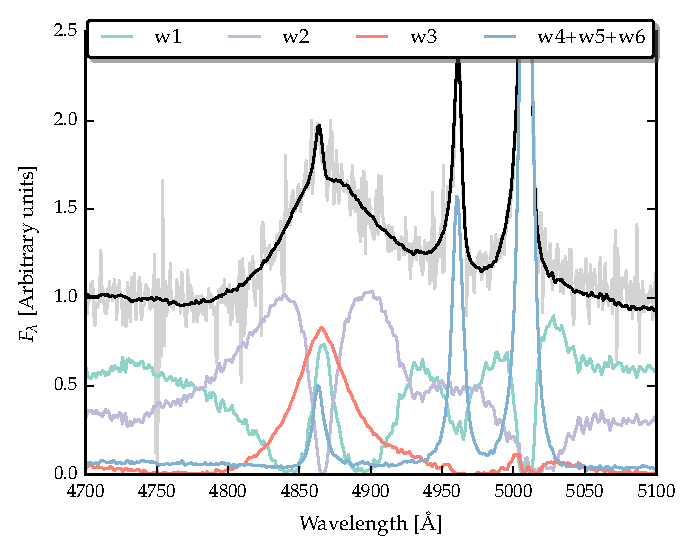
\includegraphics[width=0.8\linewidth]{figures/chapter04/mfica_components.pdf} }}
    \caption[{MFICA reconstruction of the \hbns/[\ion{O}{III}] emission in quasar J$002952$+$020607$.}]{\hbns/[\ion{O}{III}] emission in quasar J$002952$+$020607$. The MFICA reconstruction is shown in black, and the spectrum in grey. The first three components ($w_1$, $w_2$, $w_3$), and the sum of components $w_4$, $w_5$ and $w_6$ are shown individually in (a). Components $w_4$, $w_5$, $w_6$ are shown individually in (b).}     
    \label{fig:mfica_components}
\end{figure}

An example MFICA reconstruction of the \hbns/[\ion{O}{III}] emission region is shown in Figure~\ref{fig:mfica_components}. 
The shape of the individual MFICA components are highly suggestive of a relation to the underlying physical constituents of the quasar. 
This correspondence is summarised in Table~\ref{tab:icacomps}. 
The component $w_1$ corresponds to \ion{Fe}{II} emission, the components $w_2$ and $w_3$ to broad \hb emission, the components $w_4$ and $w_5$ to narrow [\ion{O}{III}] and \hb emission at the systemic redshift, and the component $w_6$ to broad, blueshifted [\ion{O}{III}] emission. 

As we show in the next section, the component weights can be used directly as a compact representation of the spectral properties. 
However, we would also like to be able to measure non-parametric emission-line properties from the high-S/N MFICA reconstruction. 
These non-parametric properties can then be readily compared to the literature. 
If MFICA components $w_4$, $w_5$ and $w_6$ (the `[\ion{O}{III}] components') comprised $100$ per cent of the [\ion{O}{III}] emission, then the [\ion{O}{III}] emission could be reconstructed by setting the `non-[\ion{O}{III}] components' ($w_1$, $w_2$ and $w_3$) to zero. 
Standard non-parametric emission properties could then be computed from the [\ion{O}{III}] reconstruction. 

In practice, a very small fraction of the [\ion{O}{III}] emission may be present in the non-[\ion{O}{III}] components because of cross-talk between the signals in the components. 
However, we can ensure that close to $100$ per cent of the [\ion{O}{III}] emission is in the [\ion{O}{III}] components by making a small adjustment to the MFICA component generation algorithm.
The non-[\ion{O}{III}] components will be generated first, with the [\ion{O}{III}] emission region interpolated across. 
With these components fixed, the [\ion{O}{III}] components, which will now include all of the [\ion{O}{III}] signal, can be generated.    

\begin{table}[t!]
  \centering
  \footnotesize 
    \begin{tabular}{cc} 
    \hline
    Component & Origin \\
    \hline
    $w_1$& \ion{Fe}{II} \\
    $w_2$& \hbns \\
    $w_3$& \hbns \\
    $w_4$& [\ion{O}{III}] core \\
    $w_5$& [\ion{O}{III}] core \\
    $w_6$& [\ion{O}{III}] wing \\
    \hline
    \end{tabular}
    \caption[{Physical interpretation of the MFICA components.}]{Physical interpretation of the MFICA components.}
  \label{tab:icacomps}
\end{table} 

\subsection{MFICA component weight distributions}

\begin{figure}
\centering 
    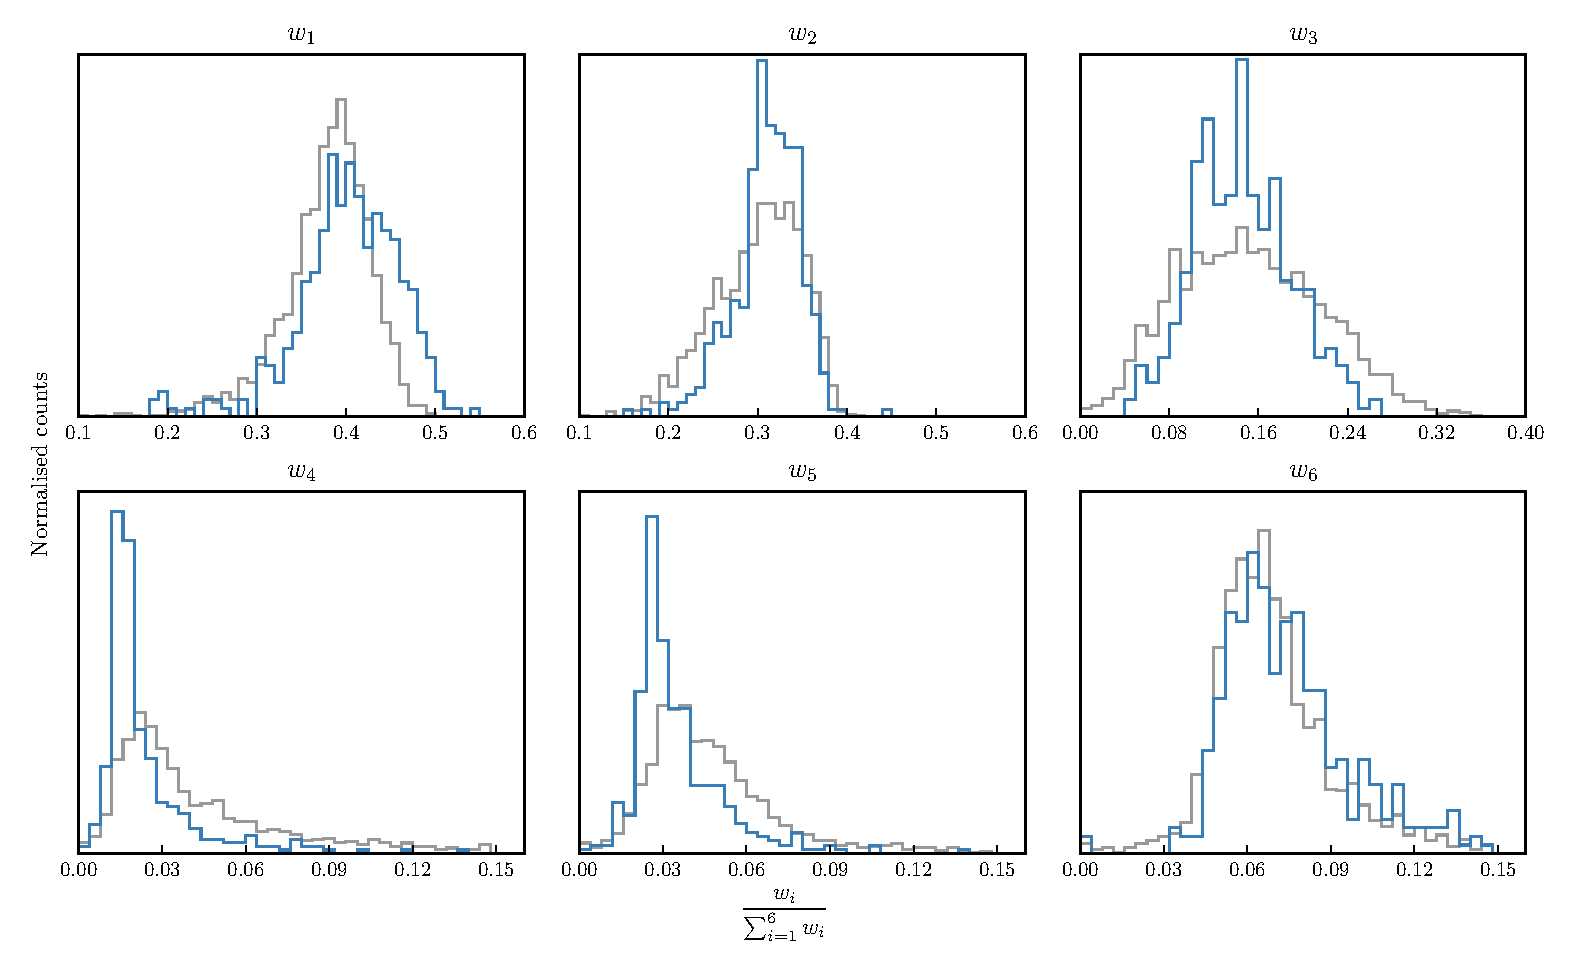
\includegraphics[width=\textwidth]{figures/chapter04/mfica_component_weights.pdf} 
    \caption[{Distributions of each of the MFICA component weights in our sample of luminous quasars and in the $z \lesssim 1$ SDSS sample.}]{Distributions of each of the MFICA component weights in our sample of luminous quasars and in the $z \lesssim 1$ SDSS sample. The core [\ion{O}{III}] emission (represented by components $w_4$ and $w_5$) is weaker in the more luminous quasar sample, but the strength of the [\ion{O}{III}] wing ($w_6$) is similar. }     
    \label{fig:mfica_component_weights}
\end{figure}

In this section, we consider how the distribution of quasars in the six-dimensional MFICA component weight parameter space changes as a function of luminosity and other quasar properties. 

Figure~\ref{fig:mfica_component_weights} shows the one-dimensional distributions of each of the MFICA component weights in our sample of luminous quasars and in the $z \lesssim 1$ SDSS sample. 
The core [\ion{O}{III}] emission (represented by components $w_4$ and $w_5$) is weaker in the more luminous quasar sample, but the strength of the [\ion{O}{III}] wing ($w_6$) is similar.
The relative weights of the core and wing components determine the overall [\ion{O}{III}] width and asymmetry, and so this demonstrates that [\ion{O}{III}] is broader and more blueshifted in the high-luminosity sample.
The same conclusions were reached in Section~\ref{sec:ch4-lumdependence}. 
The MFICA component weights suggests that the varying strength of the core component, rather than the strength of the wing, is the dominant factor in determining the overall shape of the [\ion{O}{III}] emission \citep[e.g.][]{shen14}. 

\begin{figure}
    \centering
    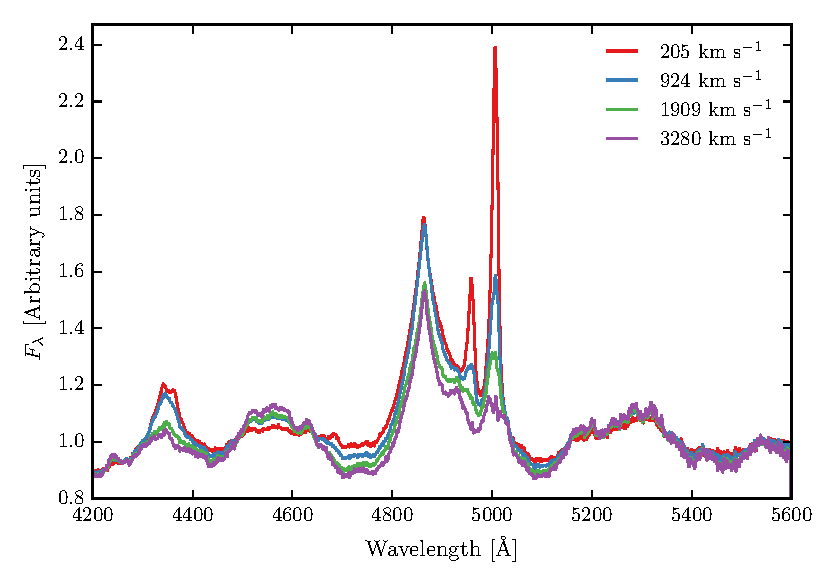
\includegraphics[width=\columnwidth]{figures/chapter04/mfica_composites.pdf} 
    \caption[{Median MFICA-reconstructed spectra as a function of the \ion{C}{IV} blueshift.}]{Median MFICA-reconstructed spectra as a function of the \ion{C}{IV} blueshift.}     
    \label{fig:mfica_composites}
\end{figure}

In Figure~\ref{fig:mfica_composites} we have taken the median MFICA component weights as a function of the \ion{C}{IV} blueshift and used these to generate high S/N representations of such spectra. 
There are strong systematic differences in the spectra as a function of the \ion{C}{IV} blueshift. 
[\ion{O}{III}] becomes progressively weaker and more blueshifted as the \ion{C}{IV} blueshift increases and in the highest \ion{C}{IV} blueshift spectrum [\ion{O}{III}] is undetected. 
The anti-correlation with the strength of \ion{Fe}{II} in the $4434$ and $4684$\,\AA\, region is also apparent. 
The same trends were previously identified in Section~\ref{sec:ch4-civtrends}.
These results demonstrate that MFICA offers a promising route forward in terms of generating high-S/N reconstructions of the observed spectra and overcoming some of the limitations of Gaussian fitting.  

The systematic difference in the spectra presented in Figure~\ref{fig:mfica_composites} (e.g. the anti-correlated strengths of [\ion{O}{III}] and \ion{Fe}{II}) are the same trends identified in the first eigenvector of the \citet{boroson92} PCA analysis (EV$1$). 
Over the years, EV$1$ has been used in attempts to explain the diversity of AGN spectra and ultimately classify AGN in the same way that the Hertzsprung–Russell diagram is used to classify stars.
Unlike the PCA eigenvectors, the MFICA components are physically interpretable, and so may prove to be a more effective means of classifying and understanding the diversity of AGN spectra. 
This is something we would like to see explored further in the future. 

\section{Summary}

The main results of this chapter are as follows: 

\begin{itemize}

\item We have analysed the [\ion{O}{III}] emission properties of $330$ quasars at redshifts ($1.5 \lesssim z \lesssim 4$) and luminosities ($45.5 \lesssim \log L_{\text{Bol}} \lesssim 49$\,\ergs). In many of these objects [\ion{O}{III}] is very broad and has a strong blueshifted component, suggesting that kilo-parsec-scale outflows in ionised gas are very common in this population. 

\item There is a strong anti-correlation between the [\ion{O}{III}] EQW and the \ion{C}{IV} blueshift. This suggests that quasar-driven winds are capable of sweeping away gas extended over kilo-parsec scales in the host galaxies. We suggest this as the cause of a factor of ten higher rate of occurrence of quasars with very weak [\ion{O}{III}] in the luminous quasar sample relative to in $z \lesssim 1$ SDSS quasars. 

\item The [\ion{O}{III}] blueshift is correlated with the \ion{C}{IV} blueshift, which could indicate a connection between gas kinematics on sub-parsec and kilo-parsec scales. On the other hand, this correlation could be induced by the core component of the [\ion{O}{III}] emission decreasing faster than the wing component, as the stable NLR gas is removed by the quasar-driven winds.  

\item We identify $18$ objects with very broad [\ion{O}{III}] emission profiles with similar characteristics to four extremely dust-reddened quasars recently identified by \citet{zakamska16}. The high fraction of these objects which are radio-loud suggests that the disturbed [\ion{O}{III}] gas kinematics could be induced by relativistic jets. 

\item The mean kinetic power of the ionised outflows is $10^{44.7}$\,\ergs, corresponding to $\sim0.15$ per cent of the bolometric luminosity. However, if the ionised outflows are accompanied by molecular outflows an order of magnitude more massive then the kinetic power may also be an order of magnitude higher, i.e. $1$ per cent of the bolometric for a typical outflow, or up to $10$ per cent for the most powerful outflows. These outflow efficiencies are in same ballpark as recent AGN feedback models, which predict a coupling efficiency between AGN-driven outflows and AGN power of $\sim5$ per cent.  

\item We use a set of ten MFICA-derived spectral components to reconstruct the rest-frame optical spectra. The corresponding set of component weights provide a compact representation of the quasar spectral properties. We show that the components correspond to physical properties, and that the distribution of component weights in the sample as a whole reveals many of the results previously brought to light using a more traditional analysis (i.e. fitting multiple Gaussian components). At the same time, with the MFICA-derived components we are able to extend our analysis to a lower S/N regime. 

\end{itemize}
 


